% TeX program = lualatex
%---------------------------ALLGEMEINE IMPORTS-------------------------------------
\documentclass[12pt,english,ngerman]{scrartcl}
\input{./protokoll_template/template.latex/input/shared_preamble.tex}

% Kopfzeile
\ihead{WS22\\
	21.12.2022} \chead{\textsc{Stark} Matthias - 12004907 \\
	\textsc{Philipp} Maximilian - 11839611}
\ohead{FLAB 1 \\
	Rasterelektronen \\
	mikroskopie}
% Fußzeile

\makeatletter
\newcommand\Autoref[1]{\@first@ref#1,@}
\def\@throw@dot#1.#2@{#1}% discard everything after the dot
\def\@set@refname#1{%    % set \@refname to autoefname+s using \getrefbykeydefault
	\edef\@tmp{\getrefbykeydefault{#1}{anchor}{}}%
	\xdef\@tmp{\expandafter\@throw@dot\@tmp.@}%
	\ltx@IfUndefined{\@tmp autorefnameplural}%
	{\def\@refname{\@nameuse{\@tmp autorefname}s}}%
	{\def\@refname{\@nameuse{\@tmp autorefnameplural}}}%
}
\def\@first@ref#1,#2{%
	\ifx#2@\autoref{#1}\let\@nextref\@gobble% only one ref, revert to normal \autoref
	\else%
		\@set@refname{#1}%  set \@refname to autoref name
		\@refname~\ref{#1}% add autoefname and first reference
		\let\@nextref\@next@ref% push processing to \@next@ref
	\fi%
	\@nextref#2%
}
\def\@next@ref#1,#2{%
	\ifx#2@ and~\ref{#1}\let\@nextref\@gobble% at end: print and+\ref and stop
	\else,~\ref{#1}% print  ,+\ref and continue
	\fi%
	\@nextref#2%
}
\makeatother

\addbibresource{raster.bib}

\begin{document}
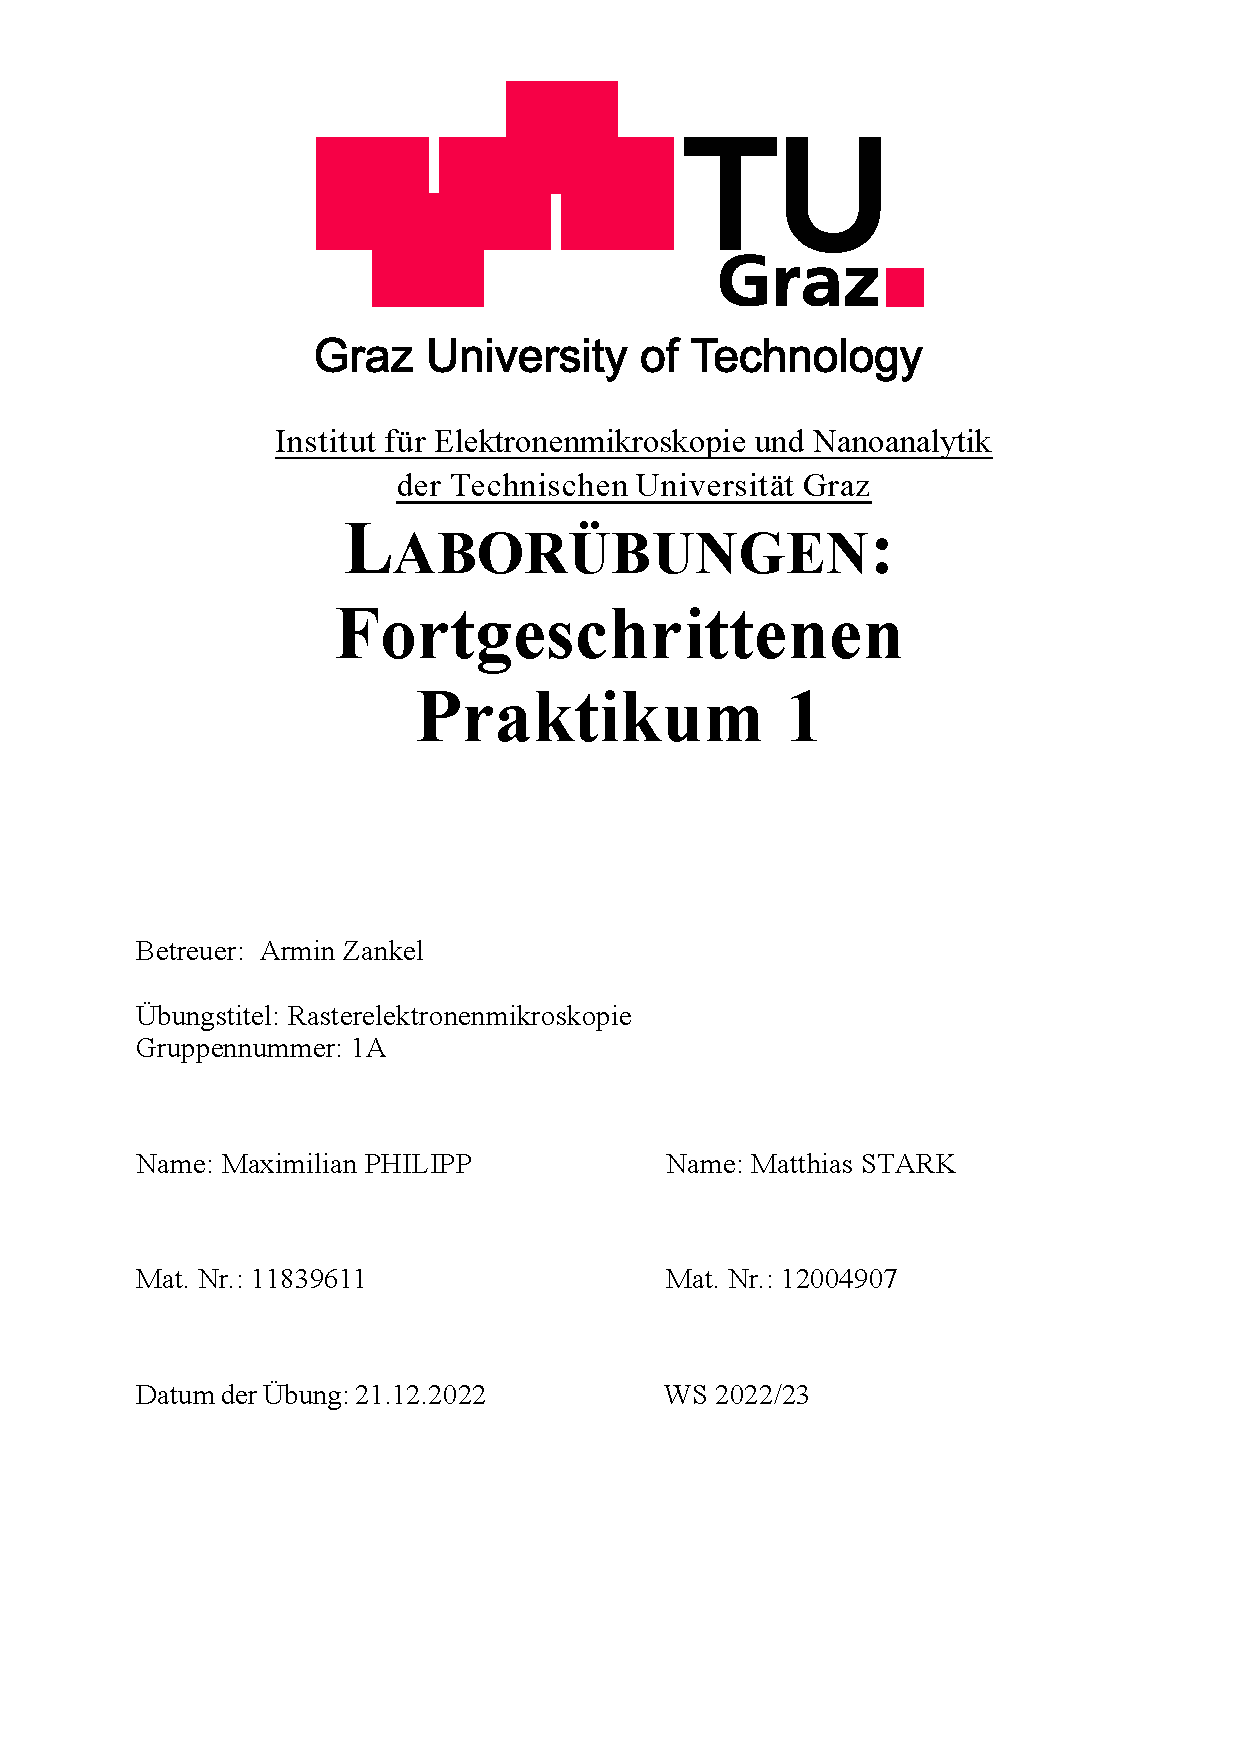
\includepdf{./deckblatt.pdf}

\section{Grundlagen}

%(max. 1 Seite)
Anmerkung: Aufgrund des großen Umfangs der Thematik der
Rasterelektronenmikroskopie, werden hier nur sehr grob die Grundlagen
skizziert. Für weiterführende Informationen, sei
auf~\cite{zankel_vorbereitungsunterlagen_2013} verwiesen, was im Anhang zu finden ist.

Rasterelektronenmikroskopie funktioniert, indem ein ein gebündelter
Elektronenstrahl auf die zu untersuchenden Proben gestrahlt wird. Dort finden
Wechselwirkungen mit dieser statt, die über die entsprechenden Detektoren
aufgefangen und als Grauwertinformation zum Bildschirm übertragen werden. Dieser
Abrastervorgang verläuft zeilenweise, bis schließlich wieder oben links begonnen
wird.

Bei den einzelnen Detektoren wird zwischen den Sekundärelektronen (SE), die
vorwiegend für Topographieuntersuchungen, Rückstreuelektronen (BSE), zur
Untersuchung der Materialeigenschaften, und Röntgenanalysen (EDX)
unterschieden.

Der grobe Aufbau eines Rasterelektronenmikroskops ist im folgenden kurz erklärt
und in \autoref{fig:aufbaurem} ersichtlich. Von der Elektronenquelle aus
werden die Elektronen zur Anode hin mit einer bestimmten
Beschleunigungsspannung ausgesendet und durch einen Aufbau von Elektronenlinsen
auf die zu untersuchende Probe hin gebündelt. Der gesamte Aufbau befindet sich
in Vakuum, um dafür zu sorgen, dass die Elektronen unterwegs nicht mit
irgendwelchen anderen Molekülen zusammentreffen oder elektrische Überschläge
stattfinden. Die Probenhalterung bietet Platz für mehrere Proben und ist in die
3 Koordinatenachsen, sowie Drehung und Rotation, bewegbar, um möglichst
effizientes Arbeiten zu ermöglichen.~\cite{zankel_vorbereitungsunterlagen_2013}

\begin{figure}[]
	\begin{center}
		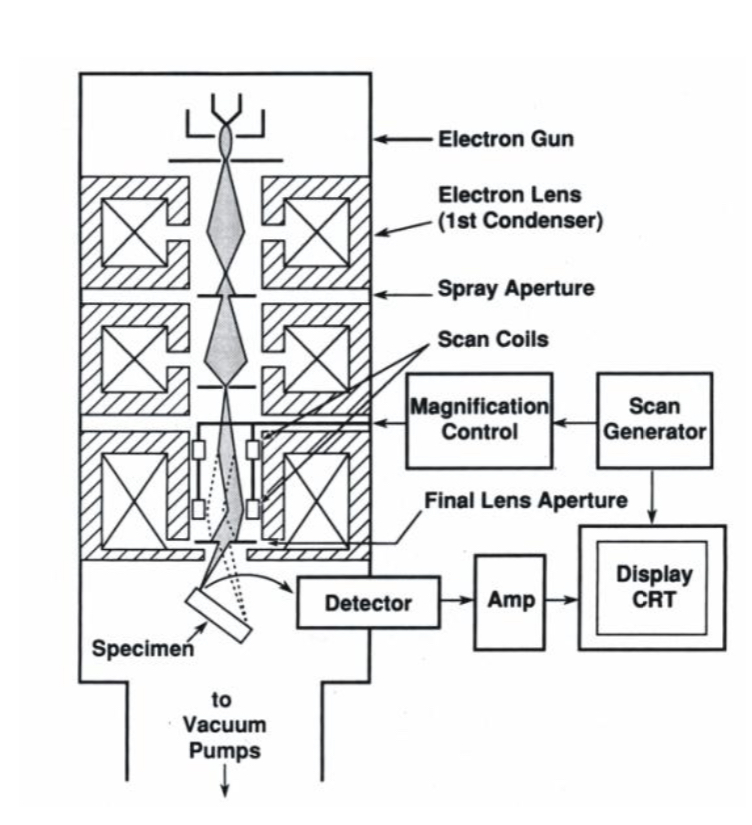
\includegraphics[width =0.5\textwidth]{./figures/aufbaurem.png}
	\end{center}
	\caption[Aufbau eines Rasterelektronenmikroskops]{Aufbau eines
		Rasterelektronenmikroskops~\cite{zankel_vorbereitungsunterlagen_2013}
	}\label{fig:aufbaurem}
\end{figure}

\section{Proben- und Geräteliste}

In folgender Aufzählung sind alle verwendeten Geräte und Materialien
aufgelistet:
\begin{itemize}
	\item Rasterelektronenmikroskop FEI ESEM Qanta 600 F
	\item EDX-Detektor (Modell: Element), der Firma EDAX
	\item Computersoftware
	\item Elektrisch leitende Probenhalter
	\item Pinzette, um die Proben einlegen zu können
	\item Doppelseitiges leitendes Kohlenstoffband, um leitende Proben befestigen zu
	      können
\end{itemize}

\newpage

Die untersuchten Proben sind in folgender Liste aufgezählt:

\begin{itemize}
	\item Heuschrecke mit Pt/Pb besputtert
	\item Polypropylen-Gewebe, teilweise C-bedampft
	\item Keramik, in Epoxidharz eingebettet, poliert und C-bedampft
	\item 10 c-Münze
\end{itemize}

\section{Kennenlernen des REM}

Zunächst wird die Probe mit einer Pinzette vorsichtig auf den Probentisch
platziert. Für ein effektives Arbeiten können mehrere Proben gleichzeitig auf
die Probenbühne gesetzt und diese zwischen den einzelnen Messungen einfach
weitergedreht werden. Im Rahmen des Praktikums wird jedoch immer nur eine Probe
eingelegt, um das Handling zu lernen und sicherzustellen, dass die ``z-Ebene'',
also die Höhe, immer richtig eingestellt ist. Die Orientierung in der
``z-Achse'' wird fixiert, um sicherzustellen, dass kein ``crash'' verursacht
wird.

Bei der Probe ist zu beachten, dass diese elektrisch leitfähig sein muss. Ist
die Probe von sich aus schon leitfähig, wird sie mit einem speziellen,
leitenden Kohlenstoff-Band am Sockel befestigt. Handelt es sich um eine nicht
leitende Probe, so muss die Leitfähigkeit z.B. durch eine Besputterung mit Platin/Palladium
gewährleistet werden, wie im \autoref{fig:probe} sichtbar.

\begin{figure}[H]
	\begin{center}
		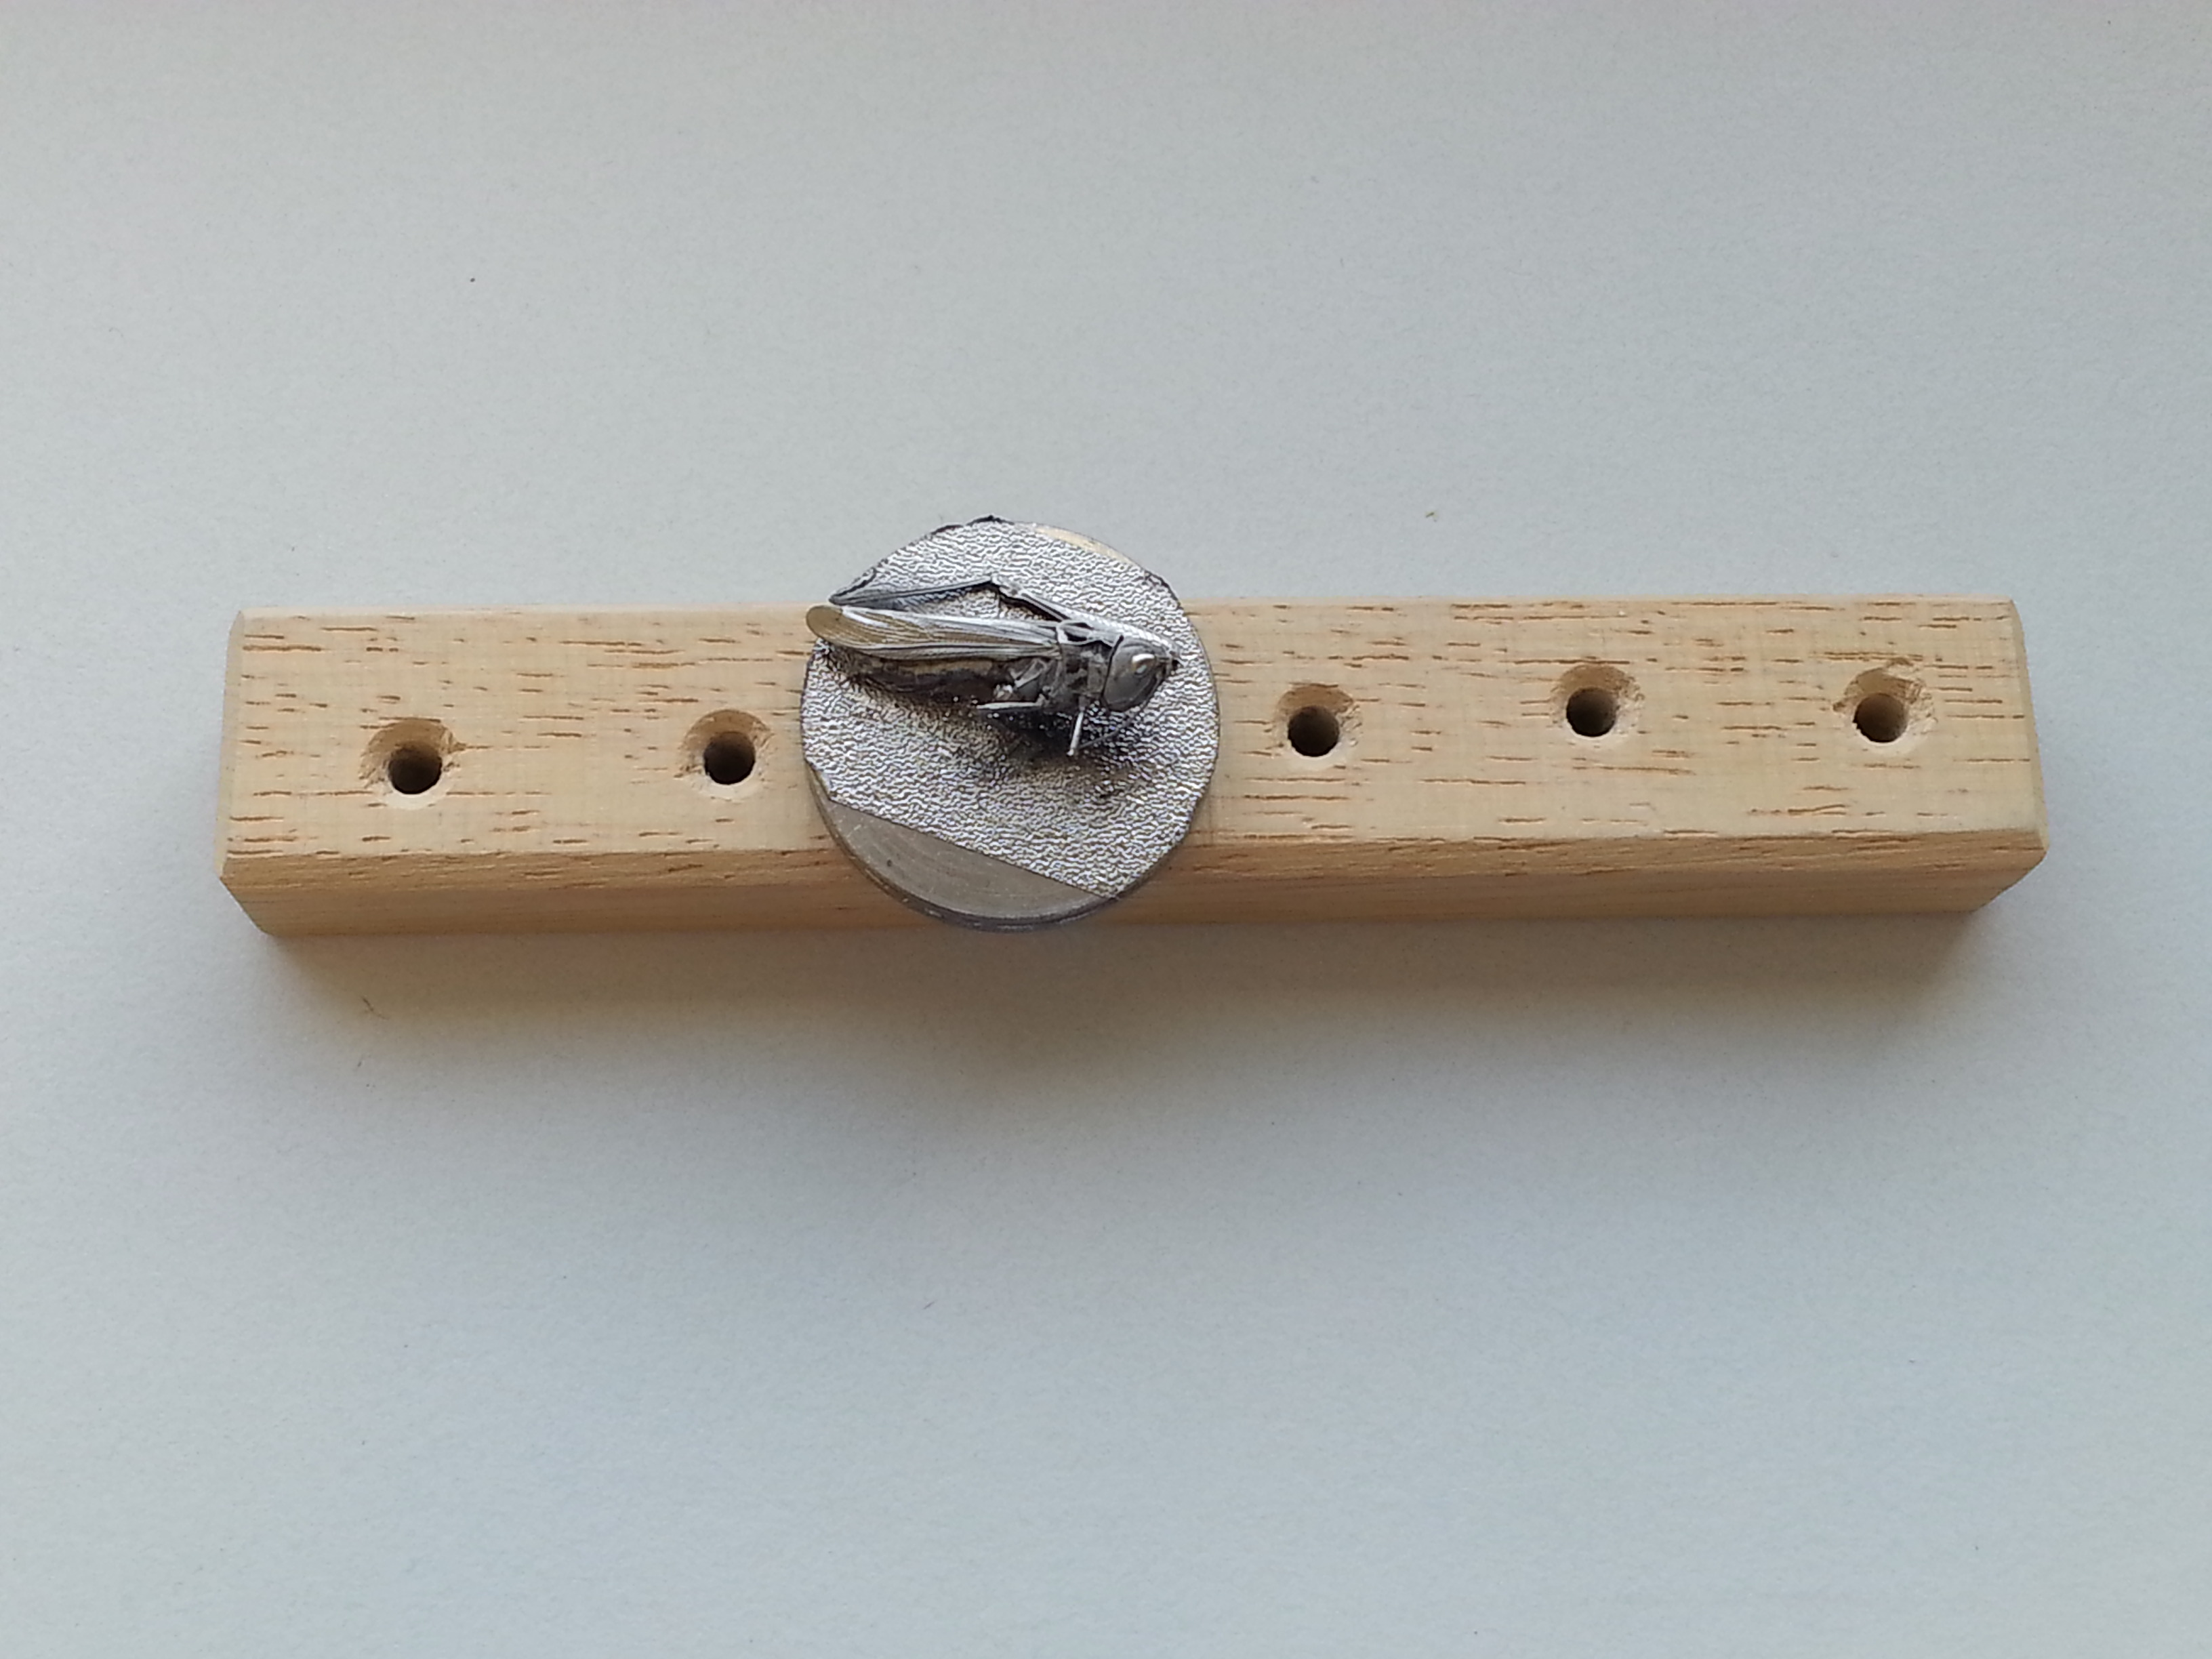
\includegraphics[width =0.5\textwidth]{./figures/probe.png}
	\end{center}
	\caption[Bedampfte, organische Probe] {Besputerter Grashüpfer,
		Probe~\cite{zankel_bedampfte_nodate}
	}\label{fig:probe}
\end{figure}

Nach dem Einlegen der Probe, die in diesem Fall einer besputterten Heuschrecke entspricht,
wird ein Vakuum erzeugt, welches für den Betrieb
des Elektronenmikroskops notwendig ist, was \SI{162(1)}{\s}, also keine
\SI{3}{\min} dauert.

Nun wird das aufgezeichnete Bild im verwendeten Computerprogramm sichtbar.
Durch Bewegung mit der Computermaus kann der entsprechende Bereich ausgewählt
und die Vergrößerung eingestellt werden. Auch kann mit der rechten Maustaste
die Schärfe, sowie mit dem entsprechenden Schiberegler in UI der Contrast und 
die Brightness, variiert werden, um ein möglichst gut
aufgelöstes Bild zu erreichen. Man muss sich bewusst sein, dass wie bei allen
optischen Aufbauten, gewisse Abbildungsfehler vorliegen. Für eine genauere
Erklärung hierzu, sein auf~\cite{zankel_vorbereitungsunterlagen_2013}
verwiesen. Der Astigmatismus kann dabei durch eine entsprechende Anpassung im jeweiligen
Menüpunkt großteils behoben werden. Zusätzlich muss auch die Grundachse richtig
ausgerichtet werden, was unter dem sogenannten ``Wobbling'' verstanden wird.

Im folgenden ist eine Auswahl der erzeugten Bilder angeführt. In
\autoref{fig:auge} sind Aufnahmen eines Facettenauges sichtbar. In
\autoref{fig:flugel} links sieht man die Struktur des Flügels und in
\autoref{fig:flugel} rechts ist eine seltsam geformte Struktur sichtbar, die
auf einen Fehler in der Bedampfungsschicht zurückzuführen ist. Generell ist zu
beachten, dass der Elektronenstrahl nicht zu lange fokussiert auf eine
bestimmte Stelle gerichtet wird, um keinen ``Beam-Damage'' zu verursachen.

\begin{figure}[H]
	\centering
	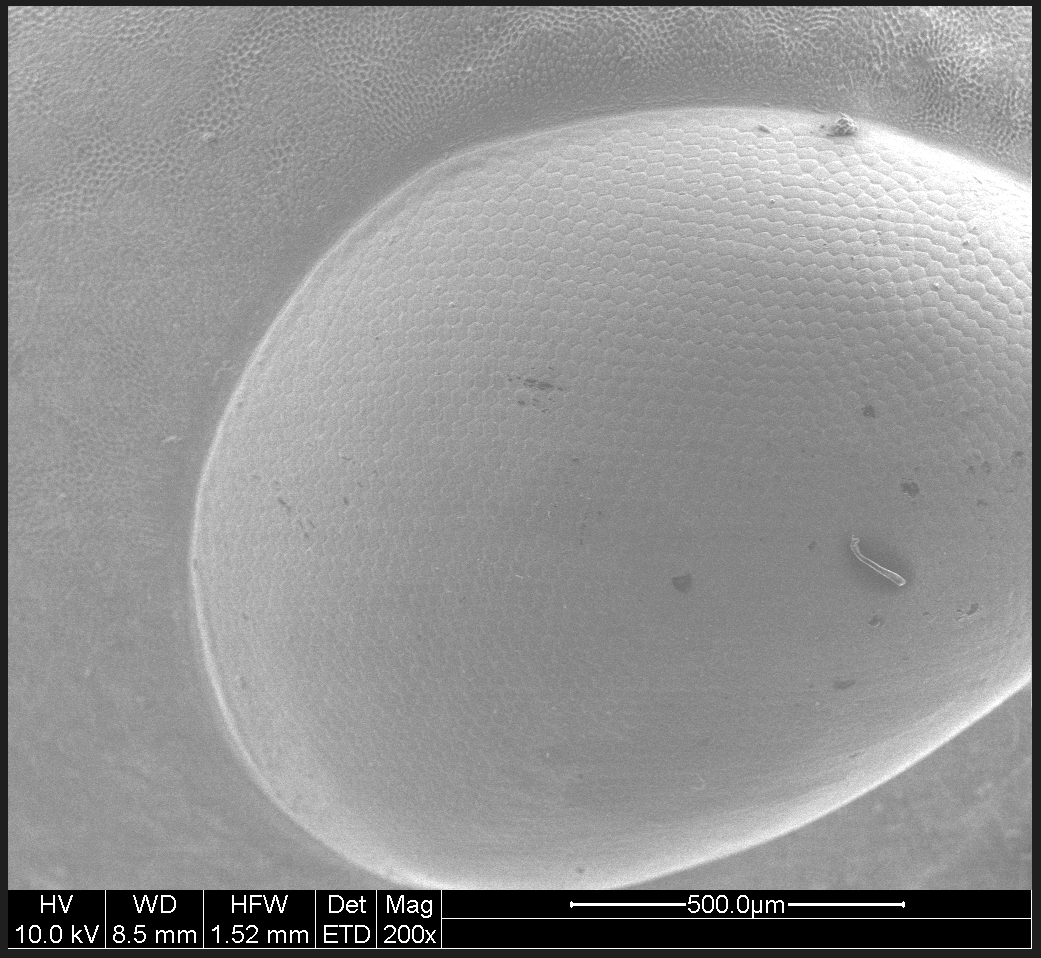
\includegraphics[width=0.48\textwidth]{./figures/auge.png}
	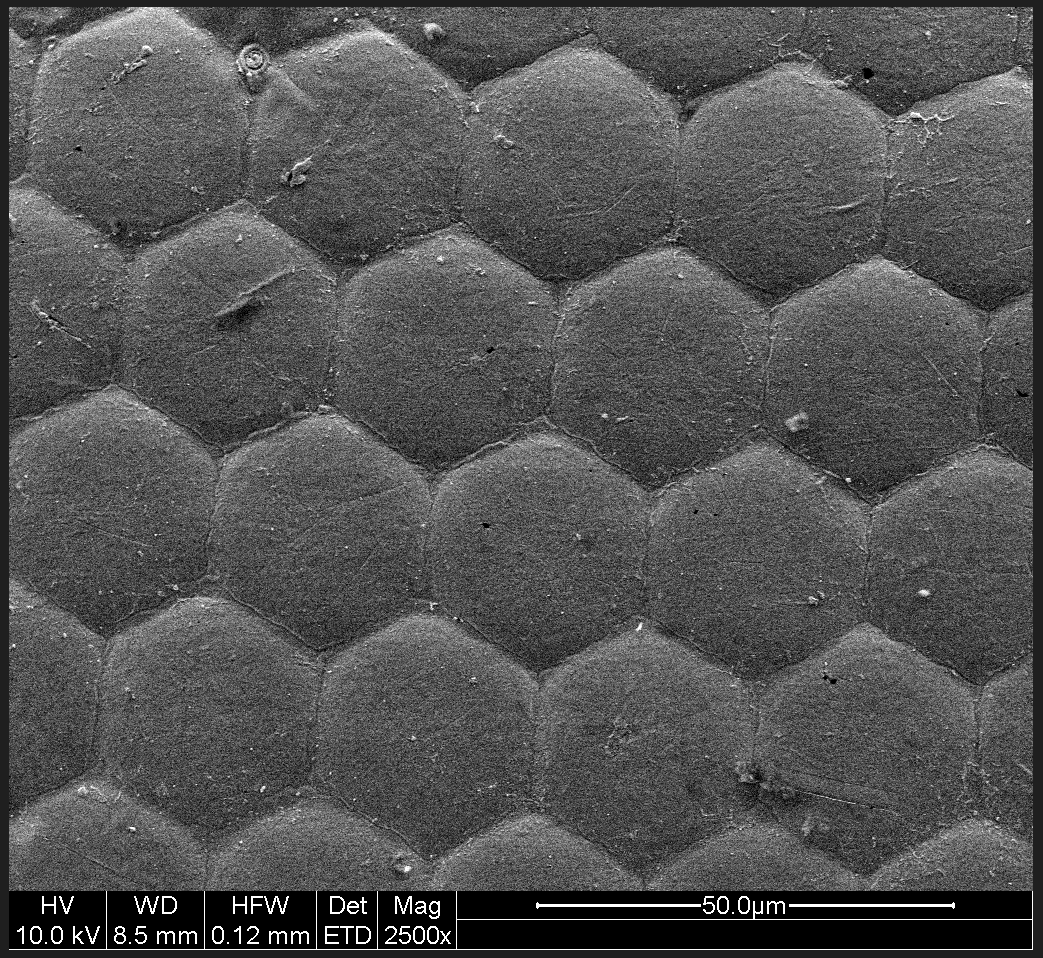
\includegraphics[width=0.48\textwidth]{./figures/auge2.png}
	\caption{Links ein makroskopisches Bild des Facettenauges eines Grashüpfers und rechts
	 ein stärker vergrößertes Bild des Facettenauges
	}\label{fig:auge}
\end{figure}

\begin{figure}[H]
	\centering
	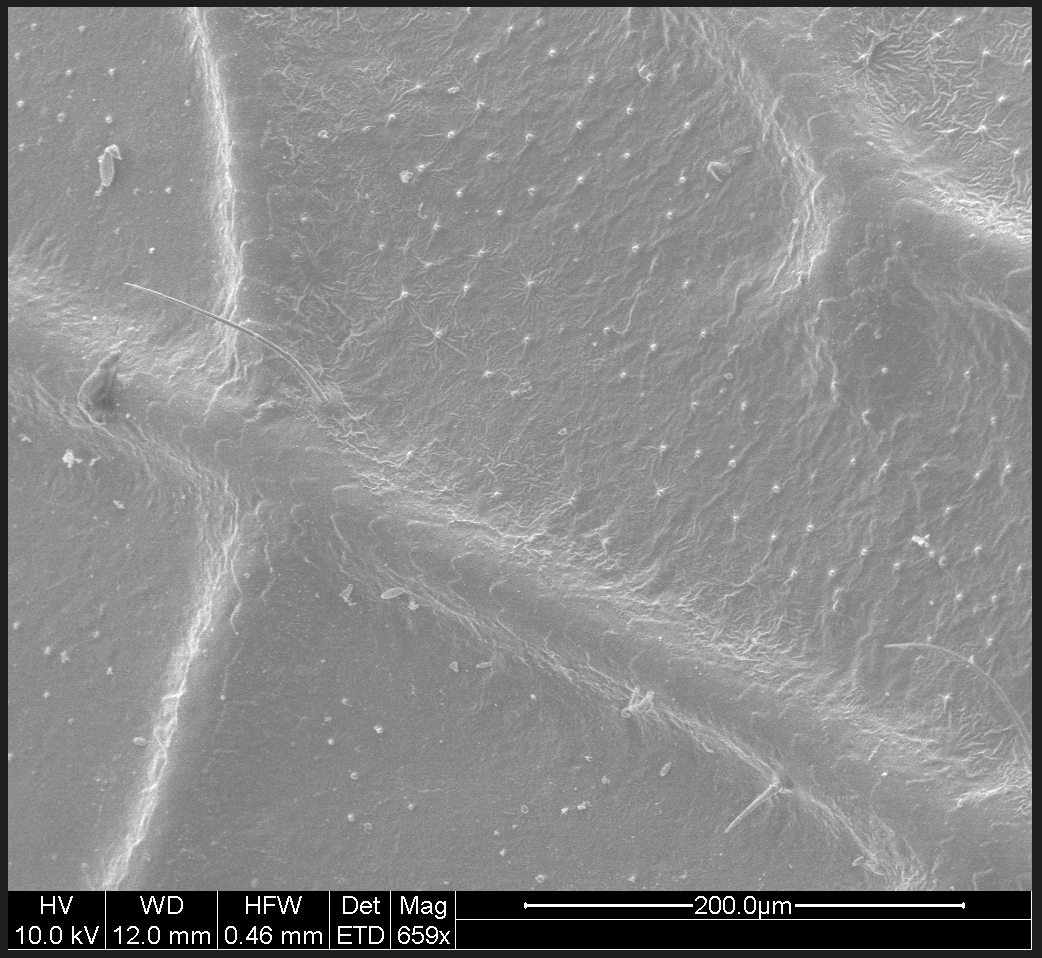
\includegraphics[width=0.48\textwidth]{./figures/flugel.png}
	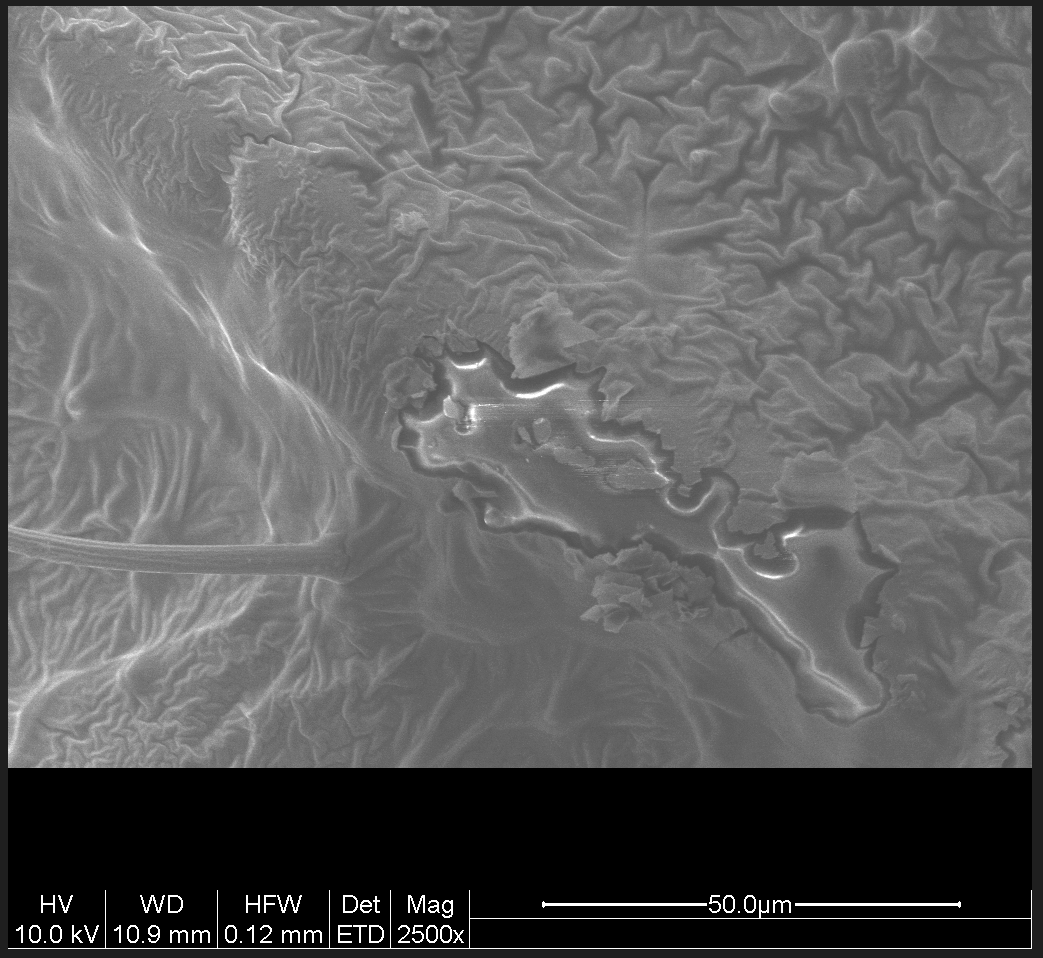
\includegraphics[width=0.48\textwidth]{./figures/damage.png}
	\caption{Links ist die Struktur des Flügels eines Grashüpfers und rechts ist ein Fehler in der Bedampfungsschicht in dieser Probe ersichtlich
	}\label{fig:flugel}
\end{figure}


Beim unbedampfte Anteil sind zeitlich fluktuierende Bewegungen ersichtlich
gewesen mehr dazu in \autoref{sec:bes_unbes}
\newpage
\section{Polypropylen-Gewebe}

Nun wird ein teilweise beschichtetes Stück eines Polypropylen-Gewebes in den
Aufbau gegeben.
%

\subsection{Vergleich „beschichtet“ und „unbeschichtet“}\label{sec:bes_unbes}

Zunächst wird jeweils eine beschichtete und eine unbeschichtete Position auf
der Probe als Position markiert, um einen unproblematischen Wechsel zwischen
ihnen zu ermöglichen. Die Betrachtung der erzeugten Bilder zeigt sofort, dass
im beschichteten Zustand viel schärfere Fotos erzeugt werden können, wie im
nächsten Kapitel ersichtlich. Betrachtet man den unbeschichteten Zustand, wie
in \autoref{fig:unbeschichtet} sichtbar, wird deutlich, dass am Präparat feine
Bewegungen der Struktur sichtbar sind, was an den ruckartigen Unterbrechungen
in folgender \autoref{fig:unbeschichtet} sichtbar wird. Besonders leicht
erkennbar werden diese Bewegungen, wenn mehrere Bilder aufgezeichnet werden und
diese dann als Film abgespielt werden, was im Rahmen dieses Protokolls aber
leider nicht geteilt werden kann.
Diese Bewegungen lassen sich dadurch erklären, dass die unbeschichtete Probe
nicht leitfähig ist und sich durch die Bestrahlung Elektronen ansammeln.
Diese Elektronenansammlung variiert durch die Bestrahlung und das elektrische
Feld, wodurch diese Fluktuationen zustande kommen.

\begin{figure}[H]
	\begin{center}
		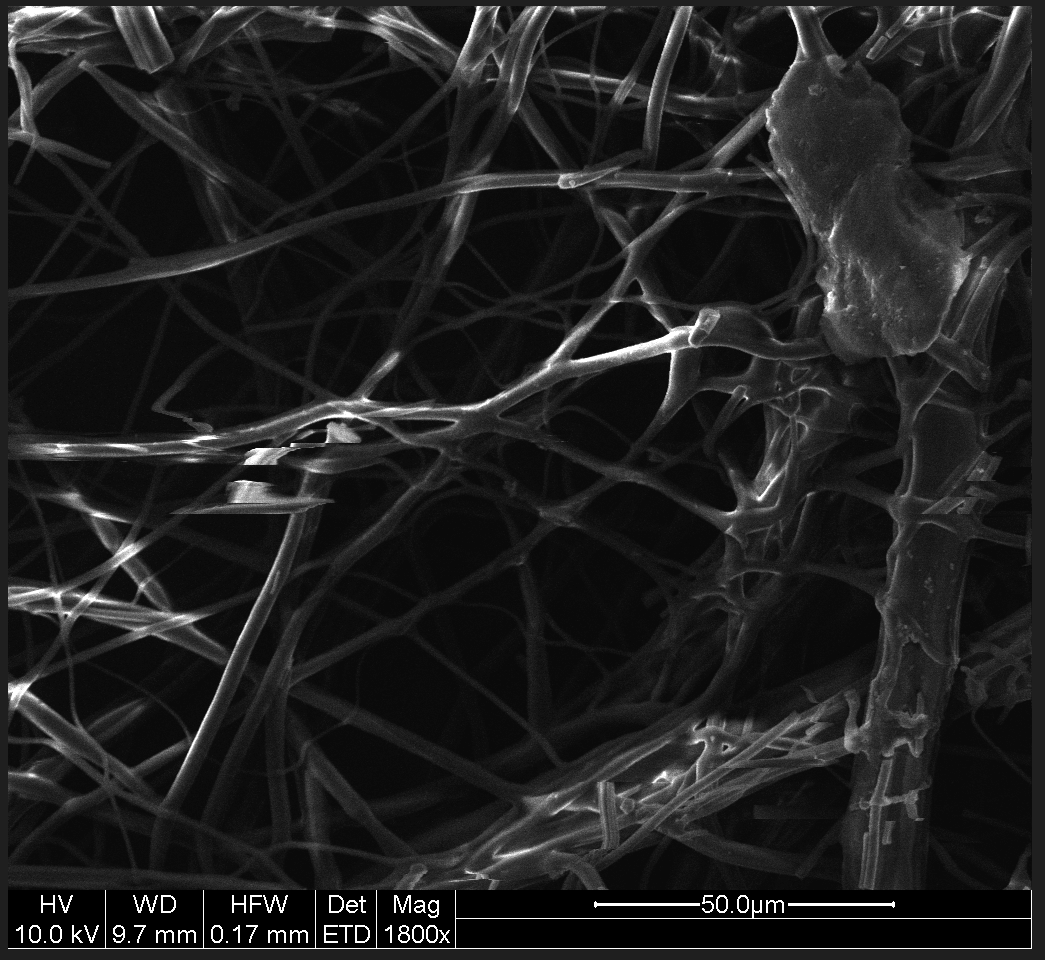
\includegraphics[width =0.5\textwidth]{./figures/unbedampft.png}
	\end{center}
	\caption{Unbeschichtetes Polypropylen-Gewebe
	}\label{fig:unbeschichtet}
\end{figure}

\subsection{Variation der Beschleunigungsspannung}

In diesem Teil des Versuchs wird die Beschleunigungsspannung der Elektronen
variiert. Wenn diese größer ist, können die Elektronen in tiefere Schichten der
Probe eindringen, weshalb die oberen, dünnen Schichten transparent wirken.
Dabei wird erwartet, dass bei der Änderung der Spannung ein Übergang zwischen 
SE und BSE zu Röngtenstrahlung sichtbar wird.

Die erzeugten Bilder sind in \autoref{fig:5kv},~\ref{fig:10kv},~\ref{fig:20kv}
und~\ref{fig:30kv} ersichtlich. Zusätzlich wurden Monte Carlo-Simulationen zur
Verfügung gestellt, die die Bewegung der Elektronen nach den Streuungen
darstellen, siehe \autoref{fig:simulation5kv},~\ref{fig:simulation10kv},~\ref{fig:simulation20kv} und~\ref{fig:simulation30kv}.

\begin{figure}[H]
	\centering
	\captionbox{SE-Bild bei einer Beschleunigungsspannung
		von \SI{5}{\kilo\volt}\label{fig:5kv}}{
		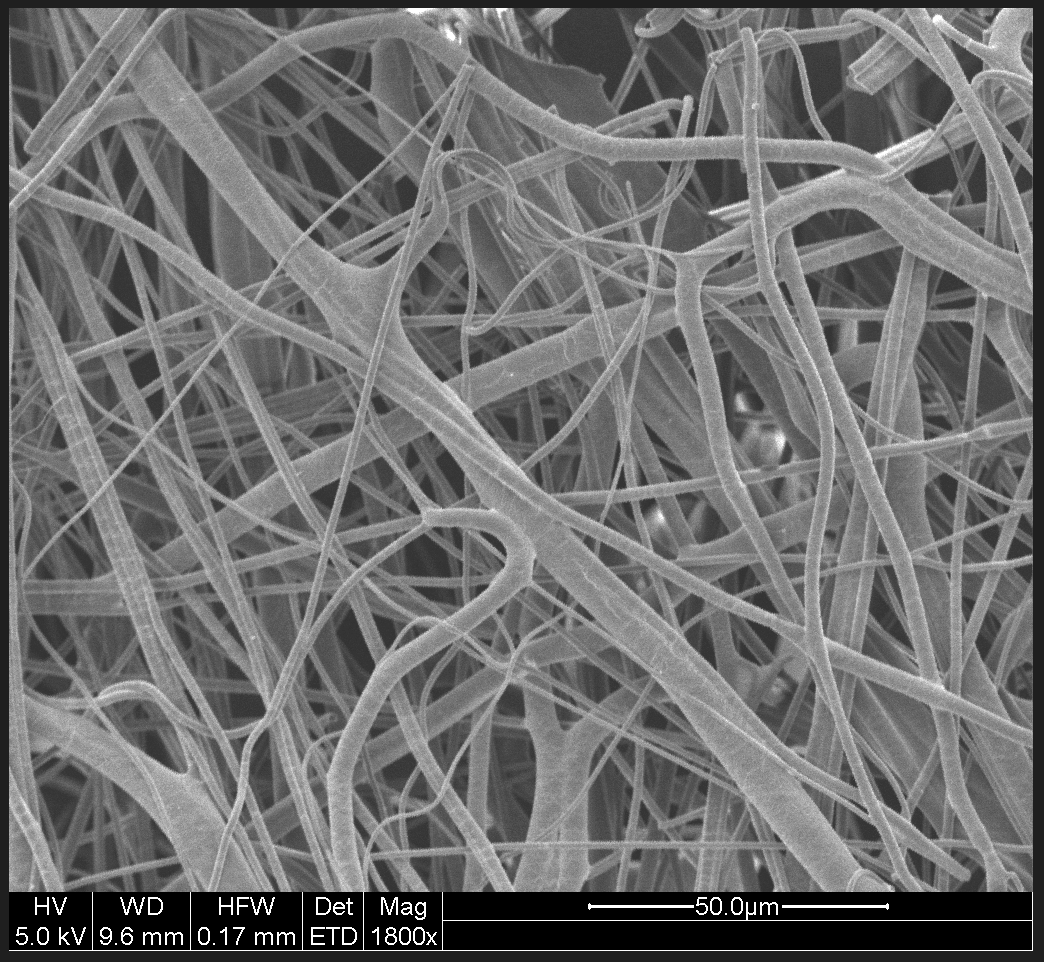
\includegraphics[width=.45\textwidth]{./figures/5kv.png}
	}
	\hfill
	\captionbox{SE-Bild bei einer Beschleunigungsspannung
		von \SI{10}{\kilo\volt}\label{fig:10kv}}{
		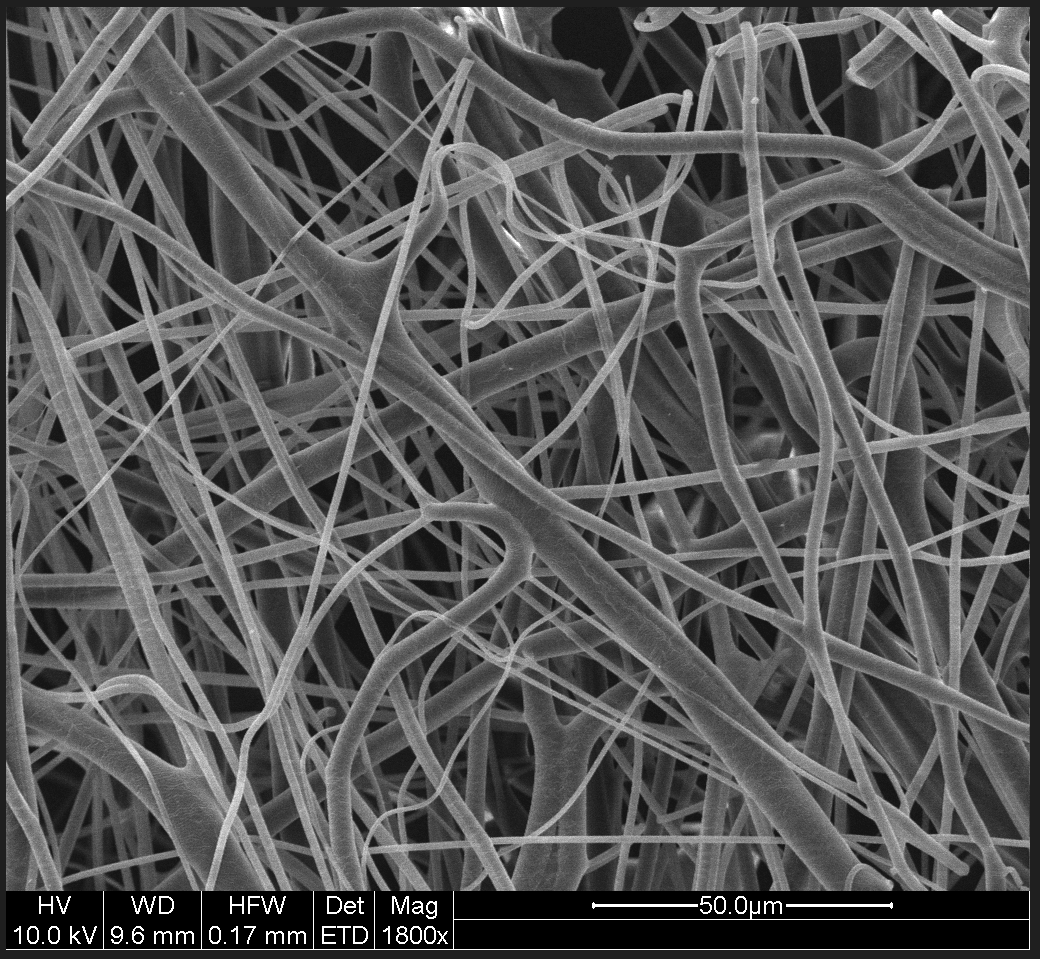
\includegraphics[width=0.45\textwidth]{./figures/10kv.png}
	}

	\captionbox{Erzeugte Simulation bei einer Beschleunigungsspannung von
		\SI{5}{\kilo\volt}~\cite{zankel_serie_nodate-1}\label{fig:simulation5kv}}{
		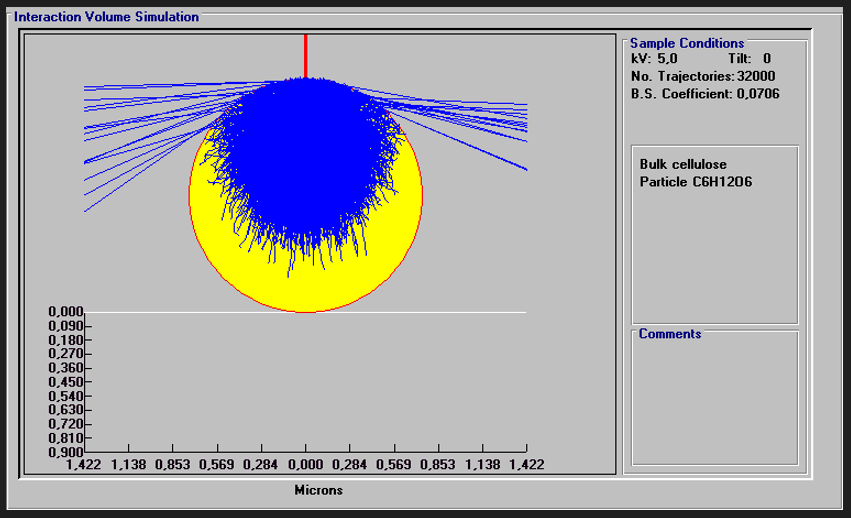
\includegraphics[width=.45\textwidth]{./figures/simulation5kv.png} } \hfill
	\captionbox{Erzeugte Simulation bei einer Beschleunigungsspannung von
		\SI{10}{\kilo\volt}~\cite{zankel_serie_nodate-1}\label{fig:simulation10kv} }{
		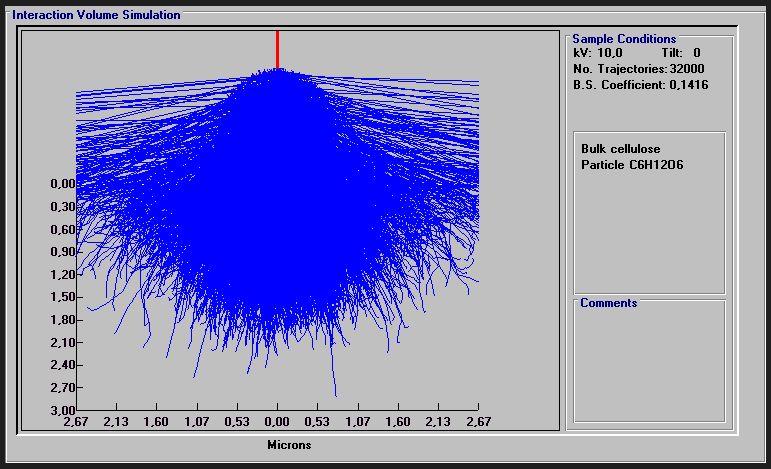
\includegraphics[width =.45\textwidth]{./figures/simulation10kv.png} }
\end{figure}

\begin{figure}[H]
	\captionbox{SE-Bild bei einer Beschleunigungsspannung
		von \SI{20}{\kilo\volt}\label{fig:20kv}}{
		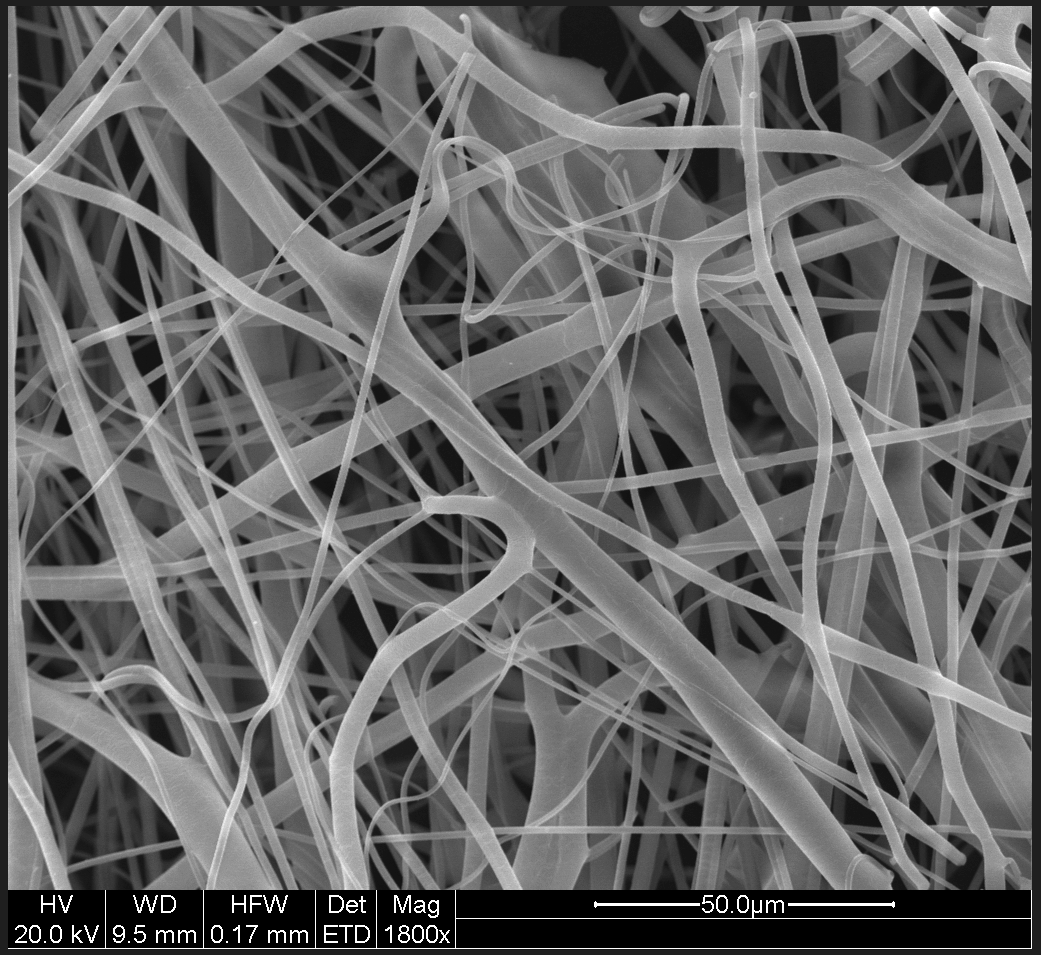
\includegraphics[width =.45\textwidth]{./figures/20kv.png} } \hfill
	\captionbox{SE-Bild bei einer Beschleunigungsspannung
		von \SI{30}{\kilo\volt}\label{fig:30kv}}{
		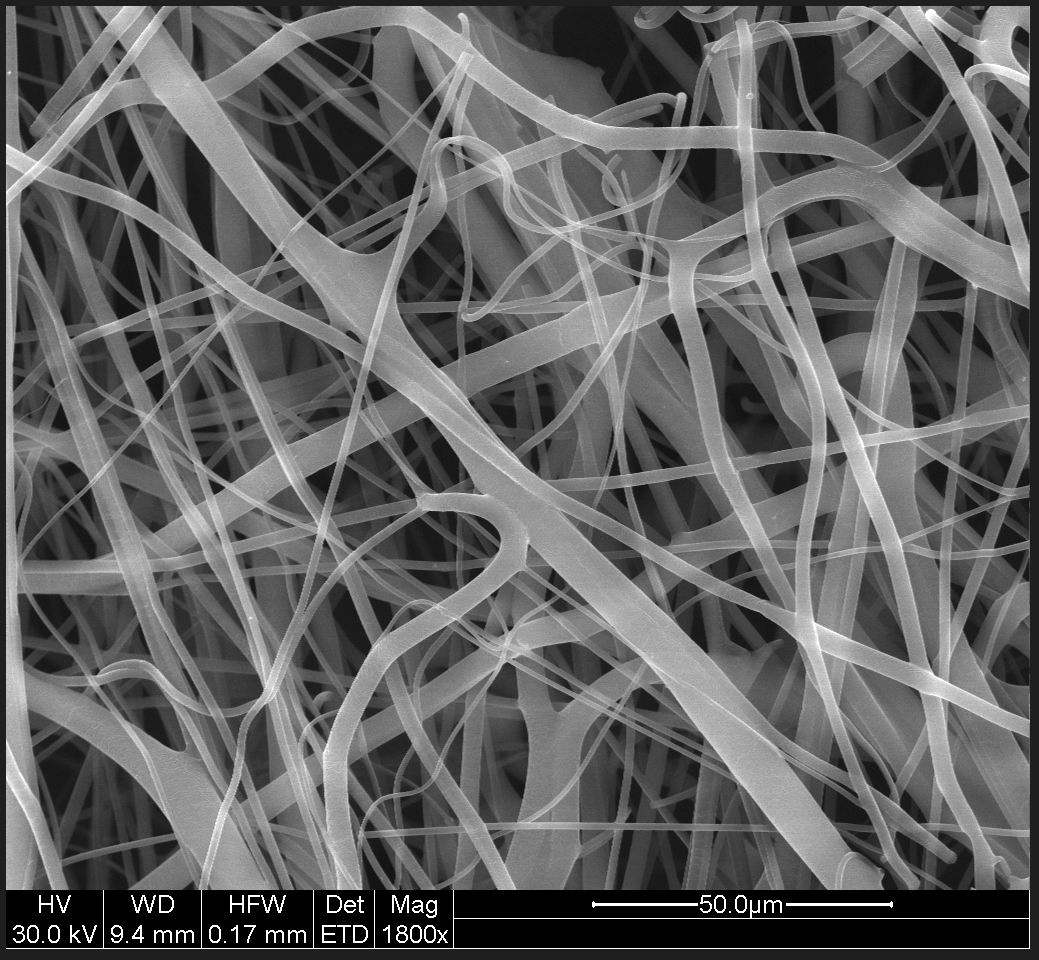
\includegraphics[width =.45\textwidth]{./figures/30kv.png}
	}

	\captionbox{Erzeugte Simulation bei einer Beschleunigungsspannung von
		\SI{20}{\kilo\volt}~\cite{zankel_serie_nodate-1}\label{fig:simulation20kv} }{
		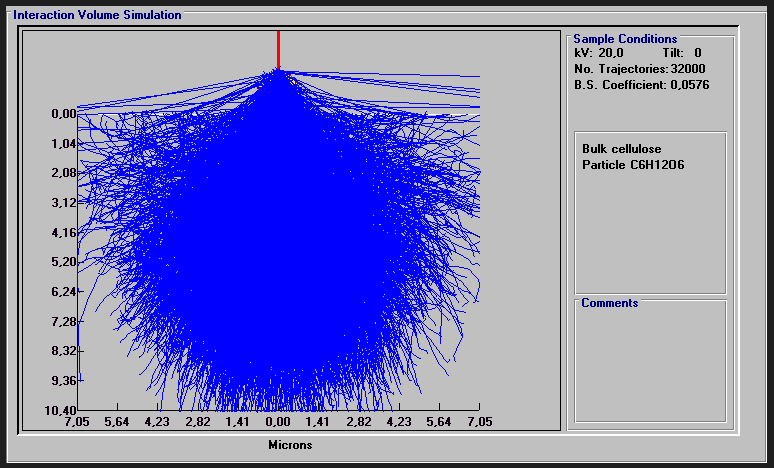
\includegraphics[width =.45\textwidth]{./figures/simulation20kv.png} } \hfill
	\captionbox{Erzeugte Simulation bei einer Beschleunigungsspannung von
		\SI{30}{\kilo\volt}~\cite{zankel_serie_nodate-1}\label{fig:simulation30kv} }{
		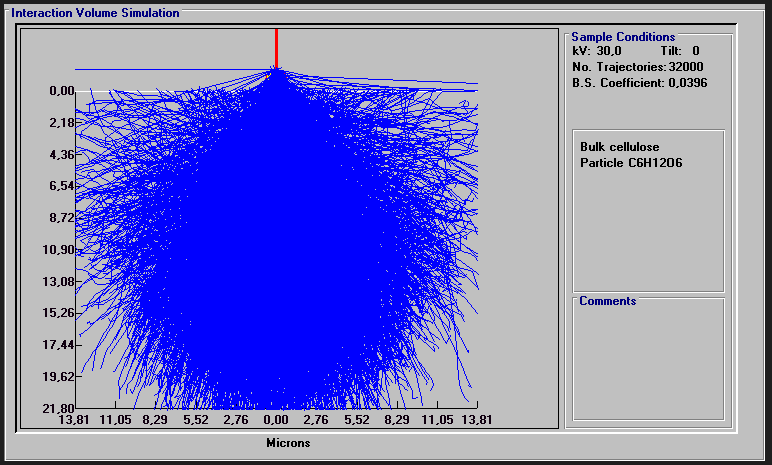
\includegraphics[width =.45\textwidth]{./figures/simulation30kv.png} }
\end{figure}

In den erzeugten SE-Bildern ist klar erkennbar, dass bei den kleinen Spannungen
besonders die Oberfläche und damit die Topografie detektiert wird. Wird die
Spannung erhöht, werden diese Feinheiten immer undeutlicher und das Bild ähnelt
immer mehr einer Röntgenaufnahme. Auch an den Simulationen ist klar
ersichtlich, dass bei der niedrigen Spannung viele Elektronen an der Oberfläche
gestreut werden und die Anderen in die Probe eindringen. Bei der höheren
Beschleunigungsspannung durchdringen diese jedoch das Gewebe, wodurch die
erkennbaren Effekte zu Stande kommen. Die SE, die großteils für die
Untersuchung der Oberflächentopografie genutzt werden, spielen bei diesem Teil
also nicht so eine große Rolle wie die BSE und die Röntgenquanten.
Im SE-Bild sind aber die Röntgenquanten nicht sichtbar und die BSE mittelbar über sogenannte SE2-Signale.

\section{Keramik}

Nun wird eine Keramikprobe in den Versuchsaufbau gegeben, wie in \autoref{fig:aufbau} sichtbar.

\begin{figure}[H]
	\begin{center}
		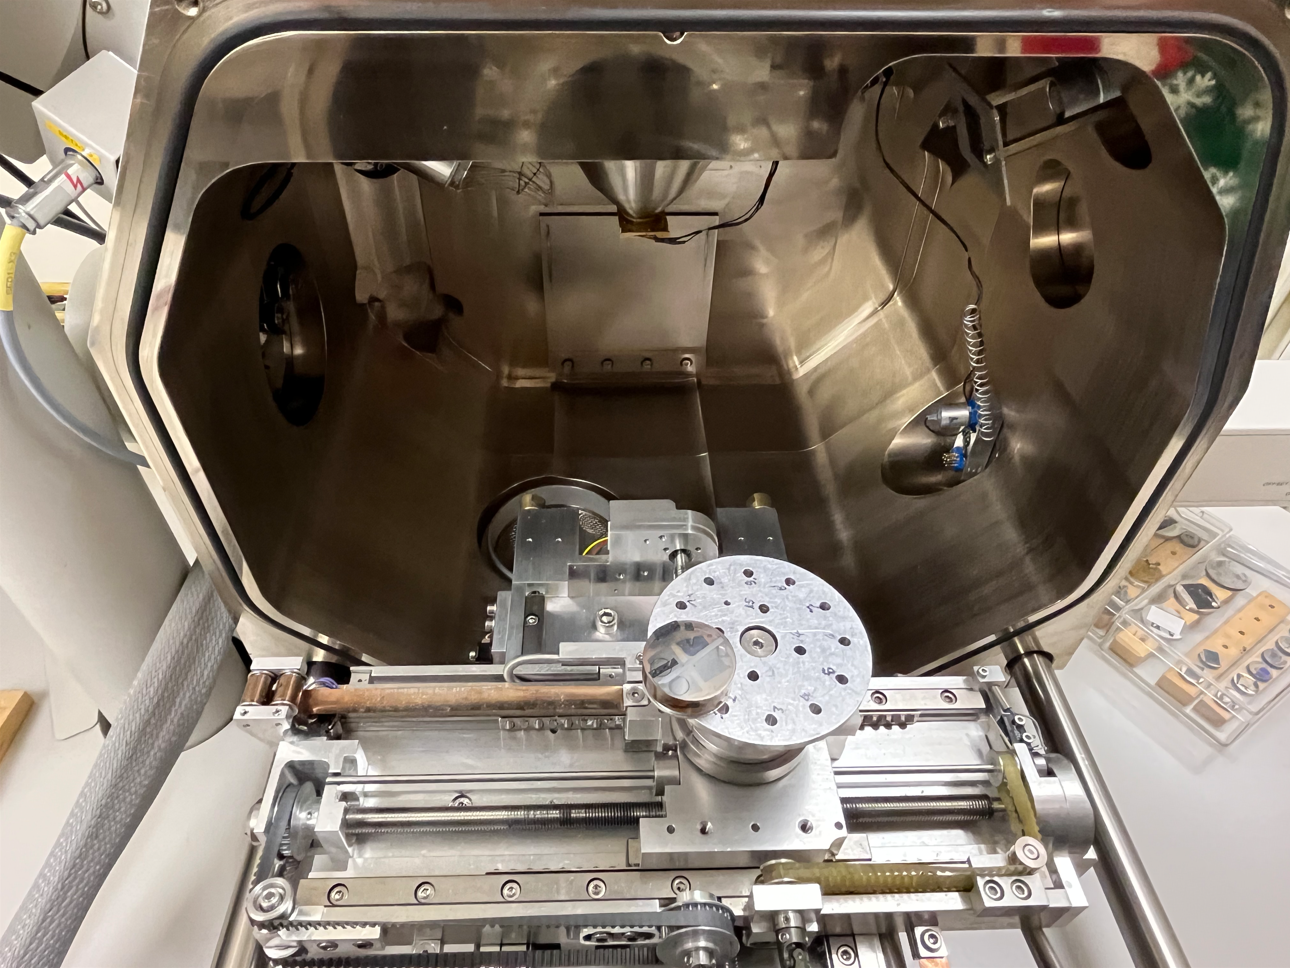
\includegraphics[width = 0.8\textwidth]{./figures/aufbau.png}
	\end{center}
	\caption{Eingebettete Keramikprobe in Versuchsaufbau
	}\label{fig:aufbau}
\end{figure}

\subsection{Vergleich SE- und BSE-Abbildung}
Bei der Keramikprobe wird nun die gleiche Position jeweils an der gleichen
Stelle nur unter Betrachtung der SE oder der BSE untersucht. Zwei so erzeugte
Bilder sind nun beispielhaft in \autoref{fig:se} und \autoref{fig:bse}
sichtbar.

\begin{figure}[H]
	\centering
	\begin{subfigure}{.45\linewidth}
		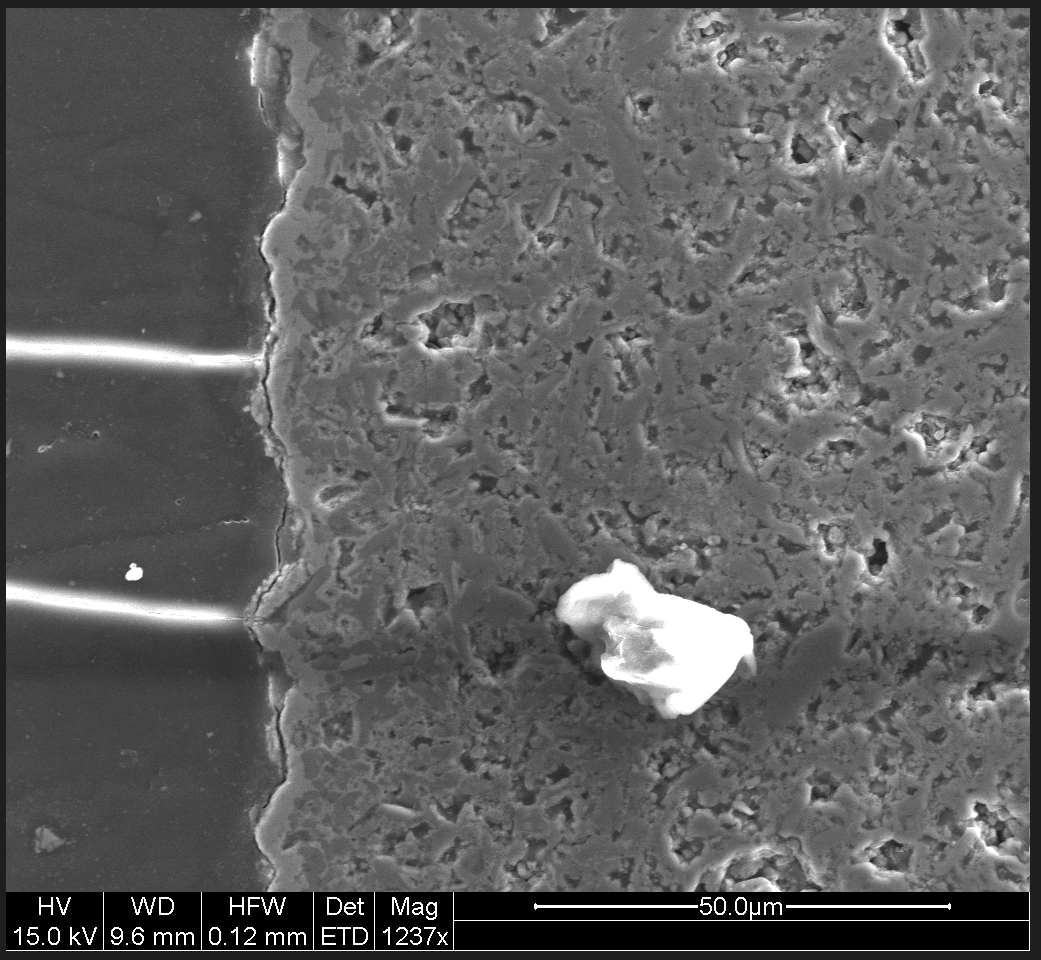
\includegraphics[width=\textwidth]{./figures/se.png}
		\caption{Erzeugtes Bild mit SE an einer Keramikprobe
		}\label{fig:se}
	\end{subfigure}
	\begin{subfigure}{.45\linewidth}
		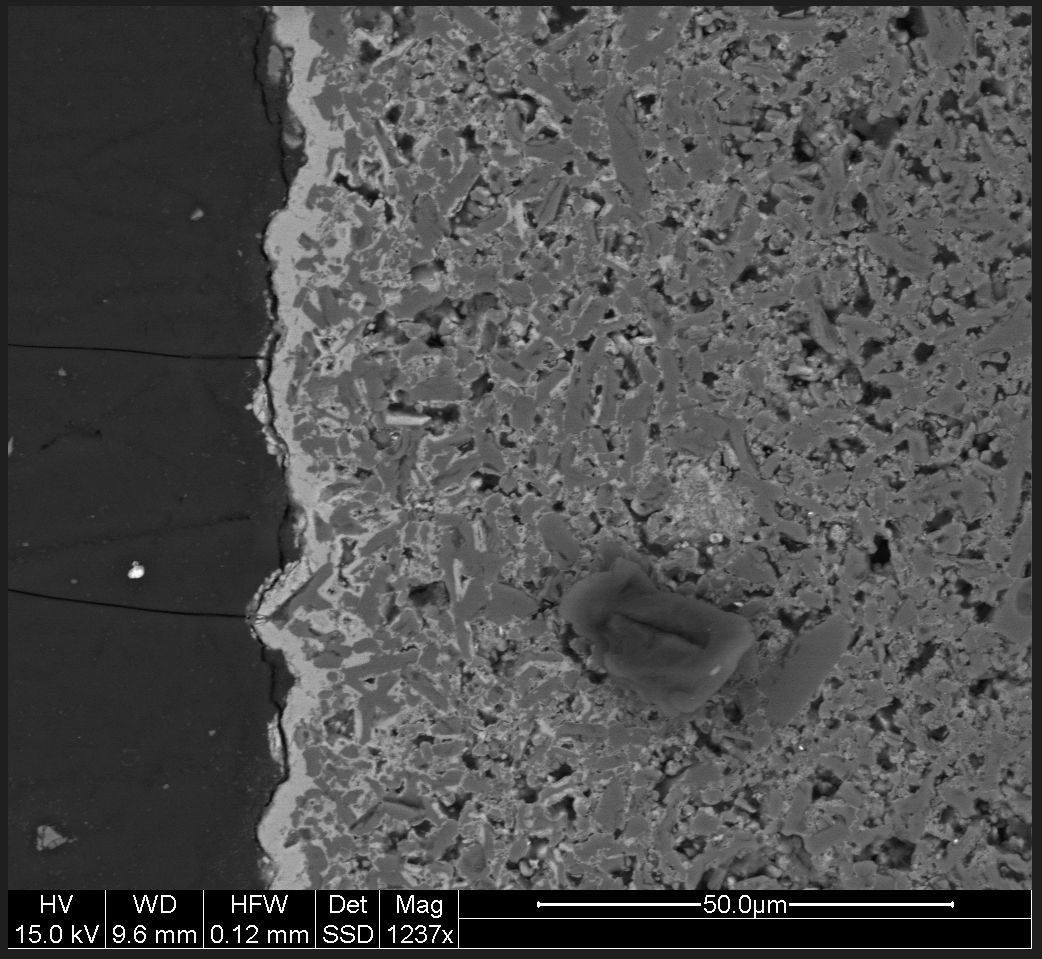
\includegraphics[width=\textwidth]{./figures/bse.png}
		\caption{Bild mit BSE an der selben Stelle der Keramikprobe
		}\label{fig:bse}
	\end{subfigure}
	\caption{Erzeugte Bilder der Keramikprobe}
\end{figure}

Es wird klar ersichtlich, dass bei dem, mit SE erzeugten Bild, insbesondere
 die Oberflächentopografie sichtbar wird, was besonders an der
Erhöhung in der Mitte des Bild erkannt werden kann. Der Grund hierfür ist, dass
diese Elektronen weniger Energie haben und daher nicht so weit in die Probe
eindringen. Die BSE dringen in die Probe ein und werden von den größeren Atomen
stärker zurückgestreut, wodurch ein stärkerer Kontrast, der sogenannte
Materialkontrast, sichtbar wird.

\subsection{Bestimmung der Schichtdicke}

Um die Schichtdicke einer Schicht auf der Keramikprobe zu bestimmen, wird am BSE-Bild die
entsprechende Schicht vermessen. Mithilfe des automatisch angezeigten Maßstabs,
kann nun die tatsächliche Schichtdicke errechnet werden. Da offensichtlich
keine homogen verteilte Dicke vorliegt, wird diese Messung für mehrere Punkte
wiederholt, wie in \autoref{fig:schichtdicke} ersichtlich. Dabei wird darauf
geachtet, immer den Abstand zu bestimmen, der möglichst orthogonal auf den Rand
der Probe liegt. Zusätzlich wurde, wie in \autoref{fig:schichtdicke}
ersichtlich, rein des Interesses halber, auch noch die Größe von
einem Keramik-Korn (grau) und einer Verunreinigung (hell)
bestimmt.

\begin{figure}[H]
	\begin{center}
		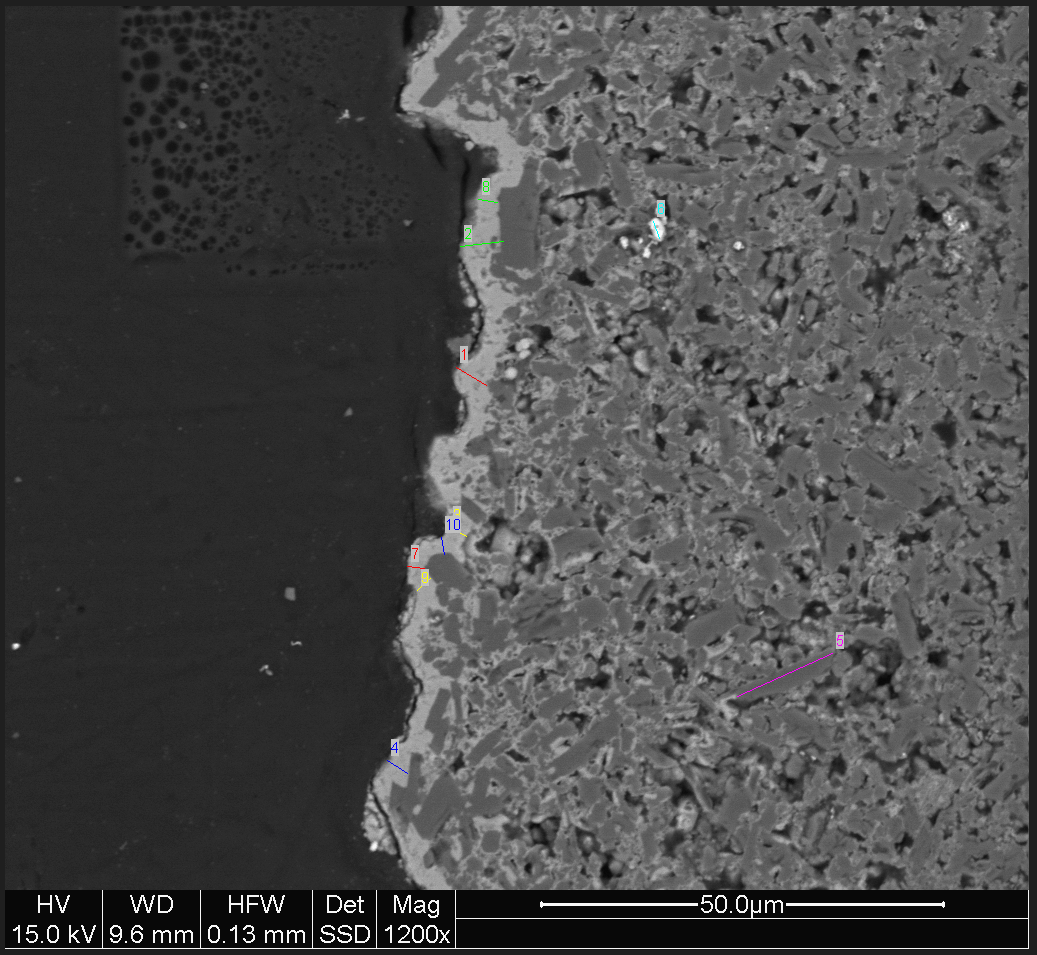
\includegraphics[width =0.8\textwidth]{./figures/schichtdicke.png}
	\end{center}
	\caption{Messung der Schichtdicke auf BSE-Bild der Keramikprobe
	}\label{fig:schichtdicke}
\end{figure}

In folgender \autoref{tab:messwerte} sind die erhaltenen Messwerte der
Schichtdicke aufgelistet. Die Unsicherheit wurde dabei als 1 Pixel angenommen,
was im konkreten Fall \SI{100}{\nano\m} entspricht.

\begin{table}[H]
	\caption[Erhaltene Messwerte für die Schichtdicke]{Erhaltene Messwerte für die
		Schichtdicke                         \\
		$m_i \dots$ entsprechender Messpunkt \\
		$d \dots$ gemessene Schichtdicke in nm mit einer Unsicherheit von \SI{100}{\nano\m}
	}
	\centering
	\begin{tabular}{|l|l|}
		\hline
		         & $d$ / nm    \\ \hline
		$m_{1}$  & \SI{4330}{} \\ \hline
		$m_{2}$  & \SI{5350}{} \\ \hline
		$m_{3}$  & \SI{2380}{} \\ \hline
		$m_{4}$  & \SI{2950}{} \\ \hline
		$m_{7}$  & \SI{2120}{} \\ \hline
		$m_{8}$  & \SI{2380}{} \\ \hline
		$m_{9}$  & \SI{2190}{} \\ \hline
		$m_{10}$ & \SI{2140}{} \\ \hline

	\end{tabular}\label{tab:messwerte}
\end{table}

%genau: 2979.14 st 1132

Aus diesen Werten ergibt sich folgende mittlere Schichtdicke $\bar{d}$ mit der
Standardabweichung $\sigma$, welche ein Maß für die Heterogenität der Schichtdicke ist:

\begin{align*}
	\bar{d} = \SI{3000}{\nano\m} \\
	\sigma = \SI{1200}{\nano\m}
\end{align*}

Für die 2 vermessenen Stellen ergeben sich folgende Durchmesser:

\begin{align*}
	d_\text{Korn} = \SI{12900(100)}{\nano\m} \\
	d_\text{Verunreinigung} = \SI{2200(100)}{\nano\m}
\end{align*}

\section{Qualitative EDX-Analyse}

Unter EDX wird ``Energy dispersive x-ray spectroscopy'' verstanden. Dies ist
eine Analysemethode, um auf die Elemente der Probe zu schließen. Dazu wird der
Elektronenstrahl auf eine bestimmte Position der Probe gerichtet. Hier werden
die entsprechenden Elektronen in den Atomen ionisiert. ``Fallen'' nun
Elektronen in die so entstandenen Löcher zurück, wird Energie frei, die in Form
von Röntgenquanten ausgestrahlt wird. Anhand dieser Quanten kann nun auf die
entsprechenden Energien und damit auf die Elemente geschlossen werden, da jedem
Element ein signifikantes Spektrum zu Grunde liegt.

Dieses Vorgehen wurde nun für die Keramikprobe an verschiedenen Positionen
wiederholt. Eine höhere Nummer der Position in \autoref{fig:position1}
-~\ref{fig:position4}, steht dabei dafür, dass die Analyse weiter innen an der
Probe durchgeführt wurde, wie in \autoref{fig:quer} sichtbar. Auch wurde nur eine Analyse der Beschichtung,
\autoref{fig:beschichtung}, und von der reinen Keramik, \autoref{fig:keramik},
durchgeführt. Da hier mit einem fokussierten Elektronenstrahl gearbeitet wird,
ist besonders darauf zu achten, keinen ``Beam-Damage'' anzurichten.

\begin{figure}[H]
	\begin{center}
		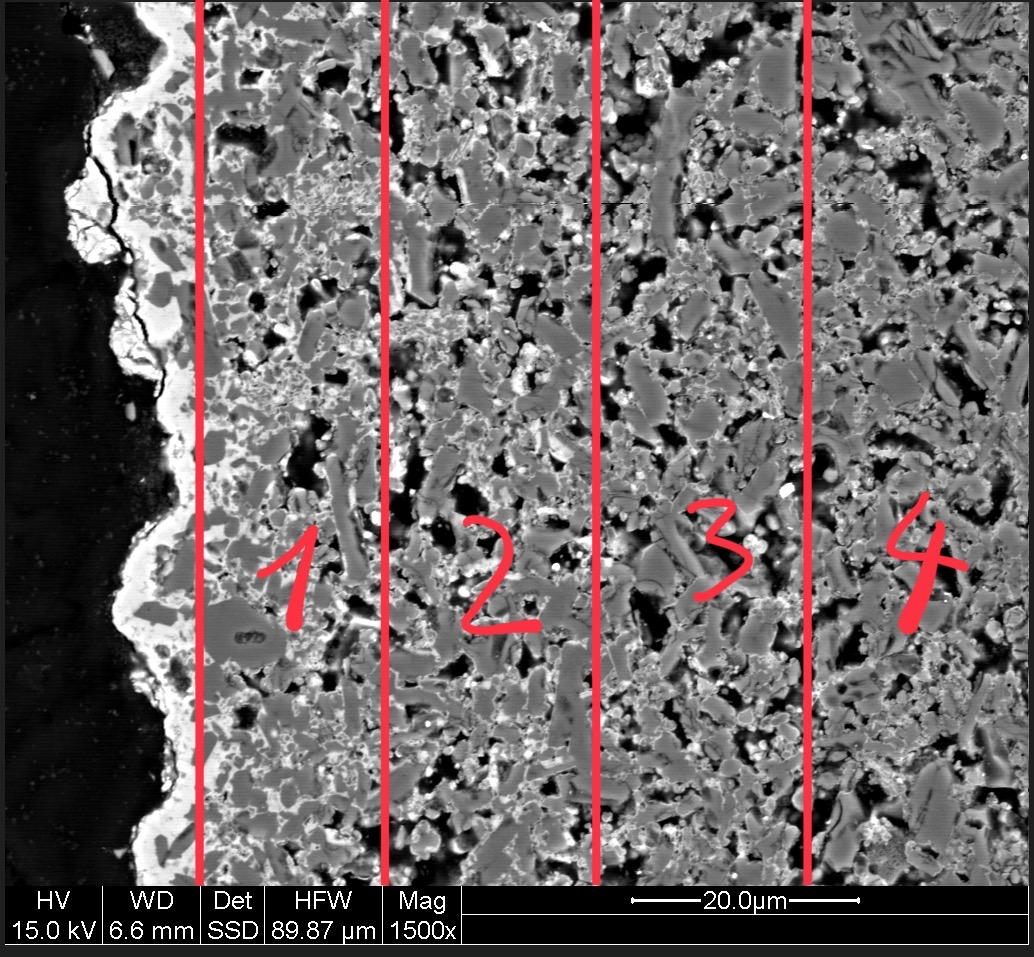
\includegraphics[width =0.5\textwidth]{./figures/querschnitt.jpg}
	\end{center}
	\caption{Keramikquerschnittes mit eingezeichneten Meßbereichen
	}\label{fig:quer}
\end{figure}

\begin{figure}[H]
	\begin{center}
		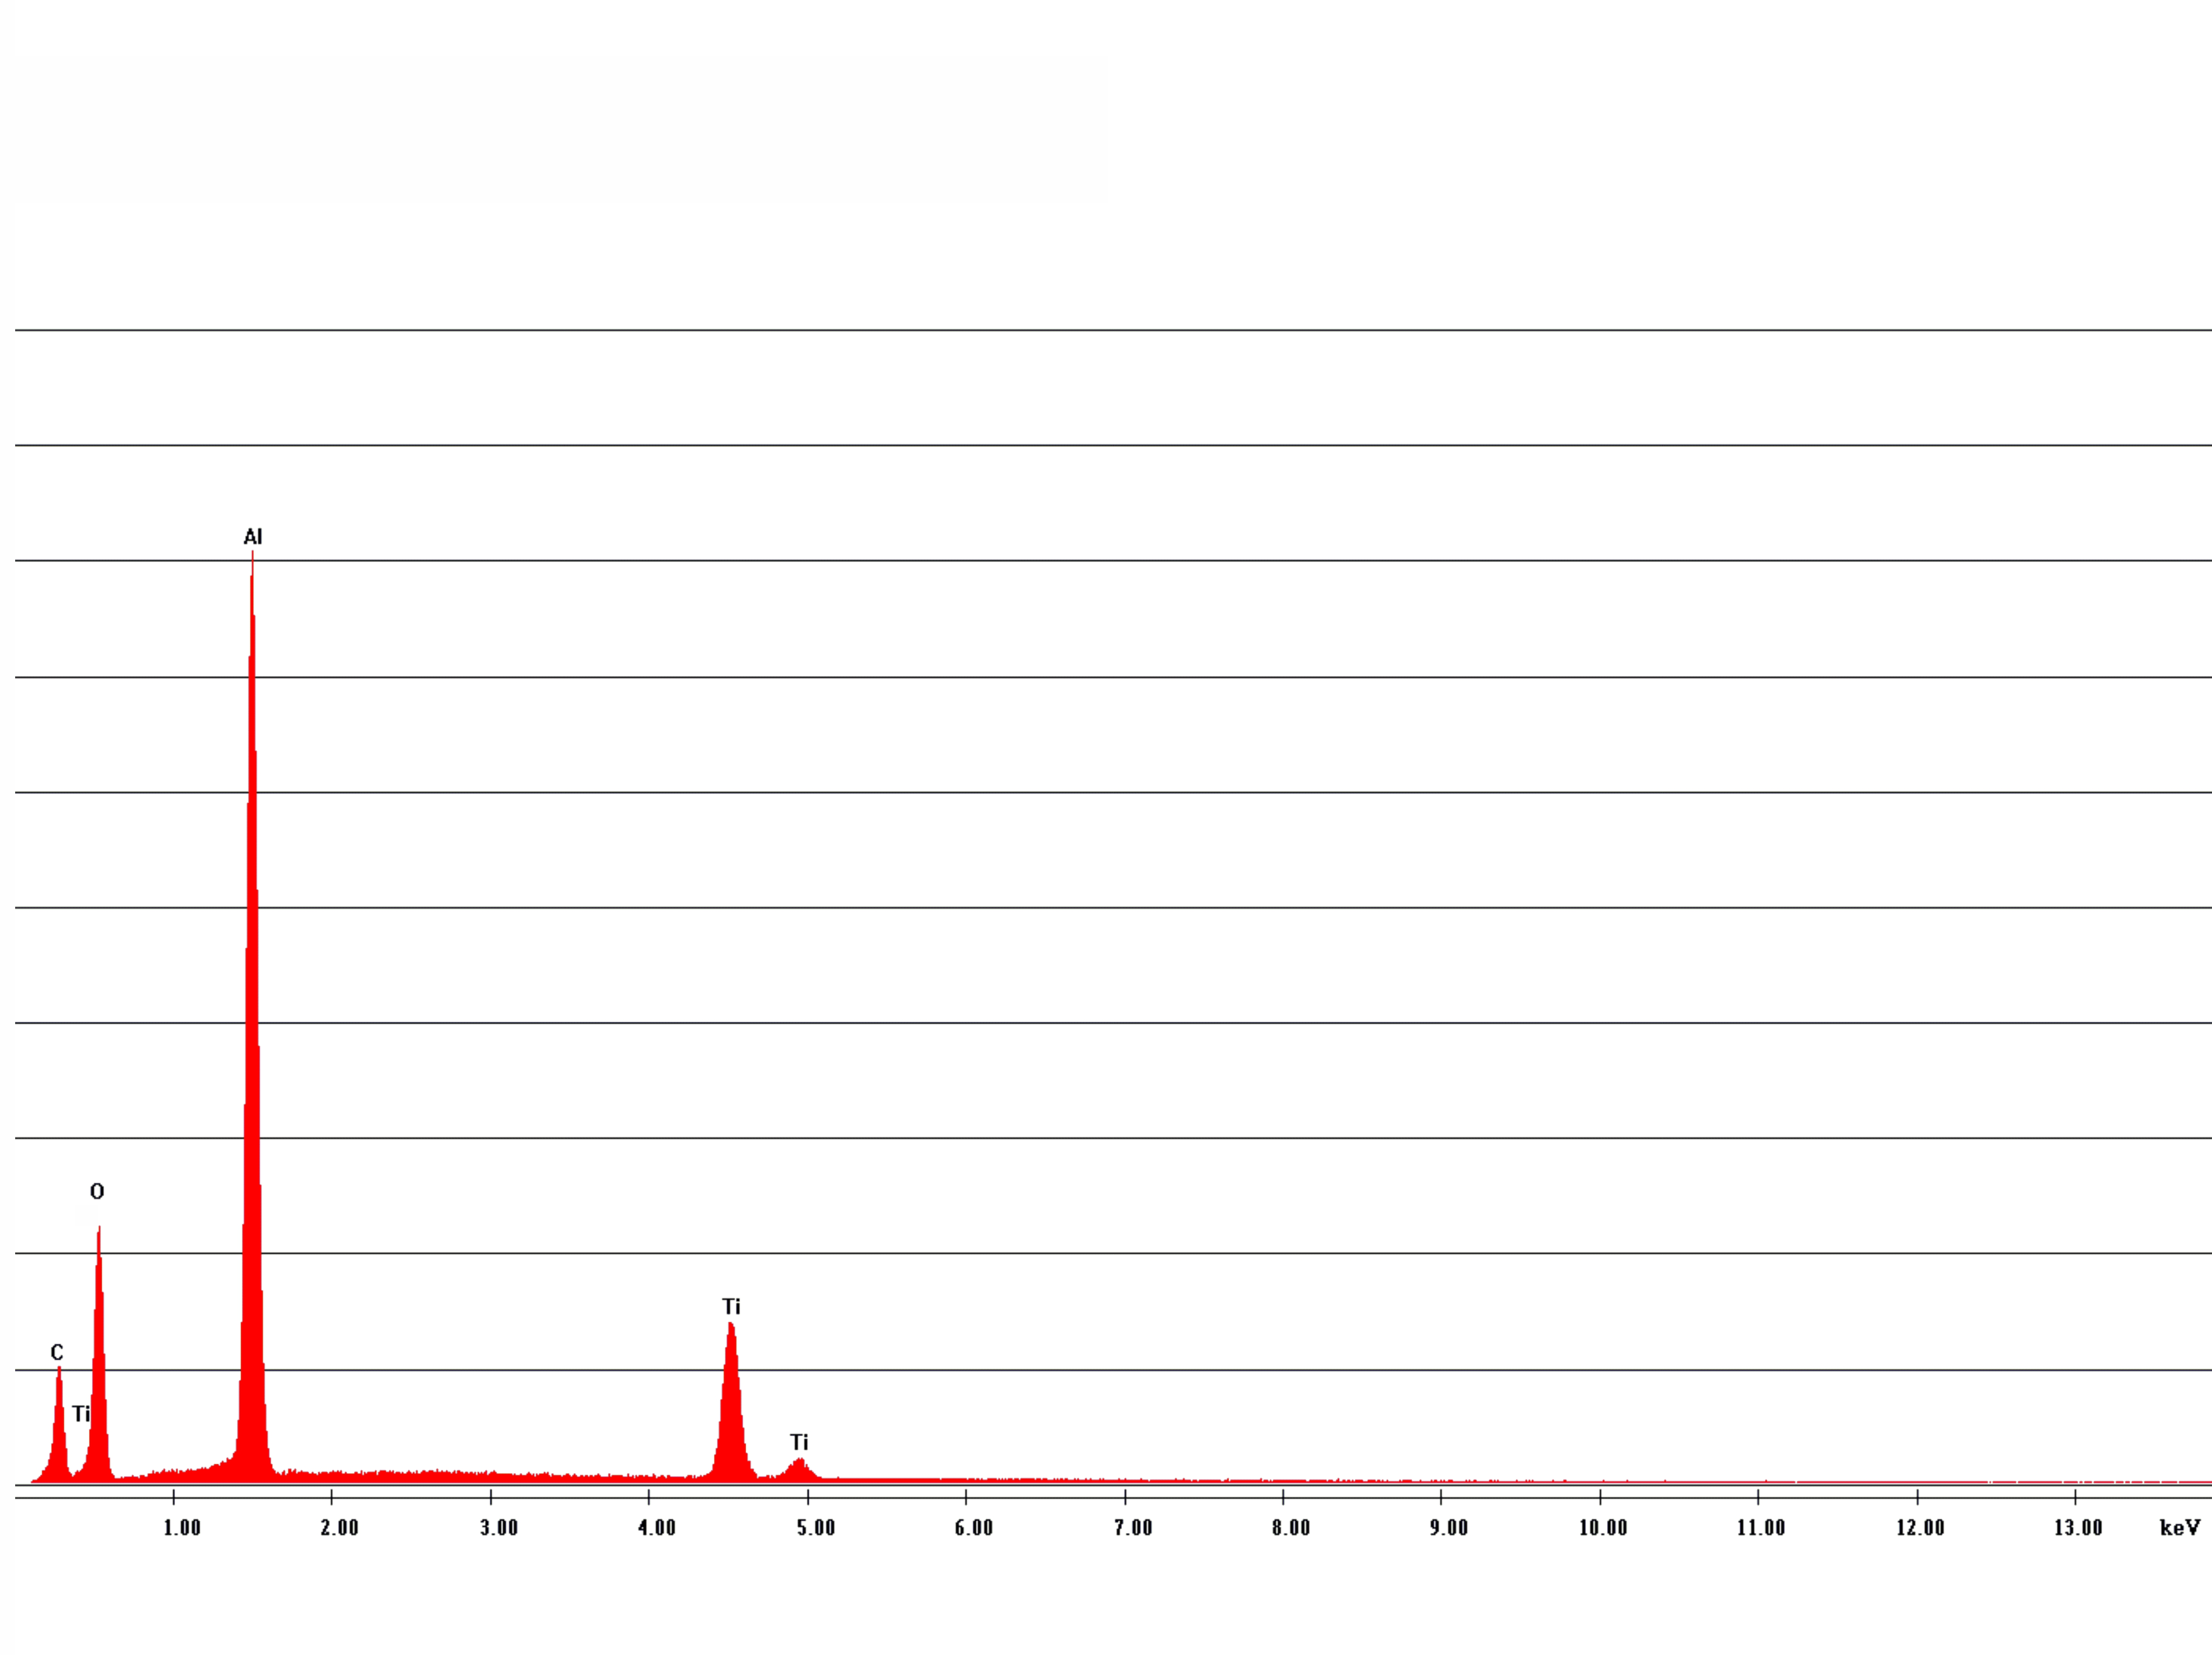
\includegraphics[width =\textwidth,height=5.3cm]{./figures/edx1.png}
	\end{center}
	\caption{EDX-Analyse der Keramikprobe an Position 1~\cite{zankel_serie_nodate}
	}\label{fig:position1}
\end{figure}
\begin{figure}[H]
	\begin{center}
		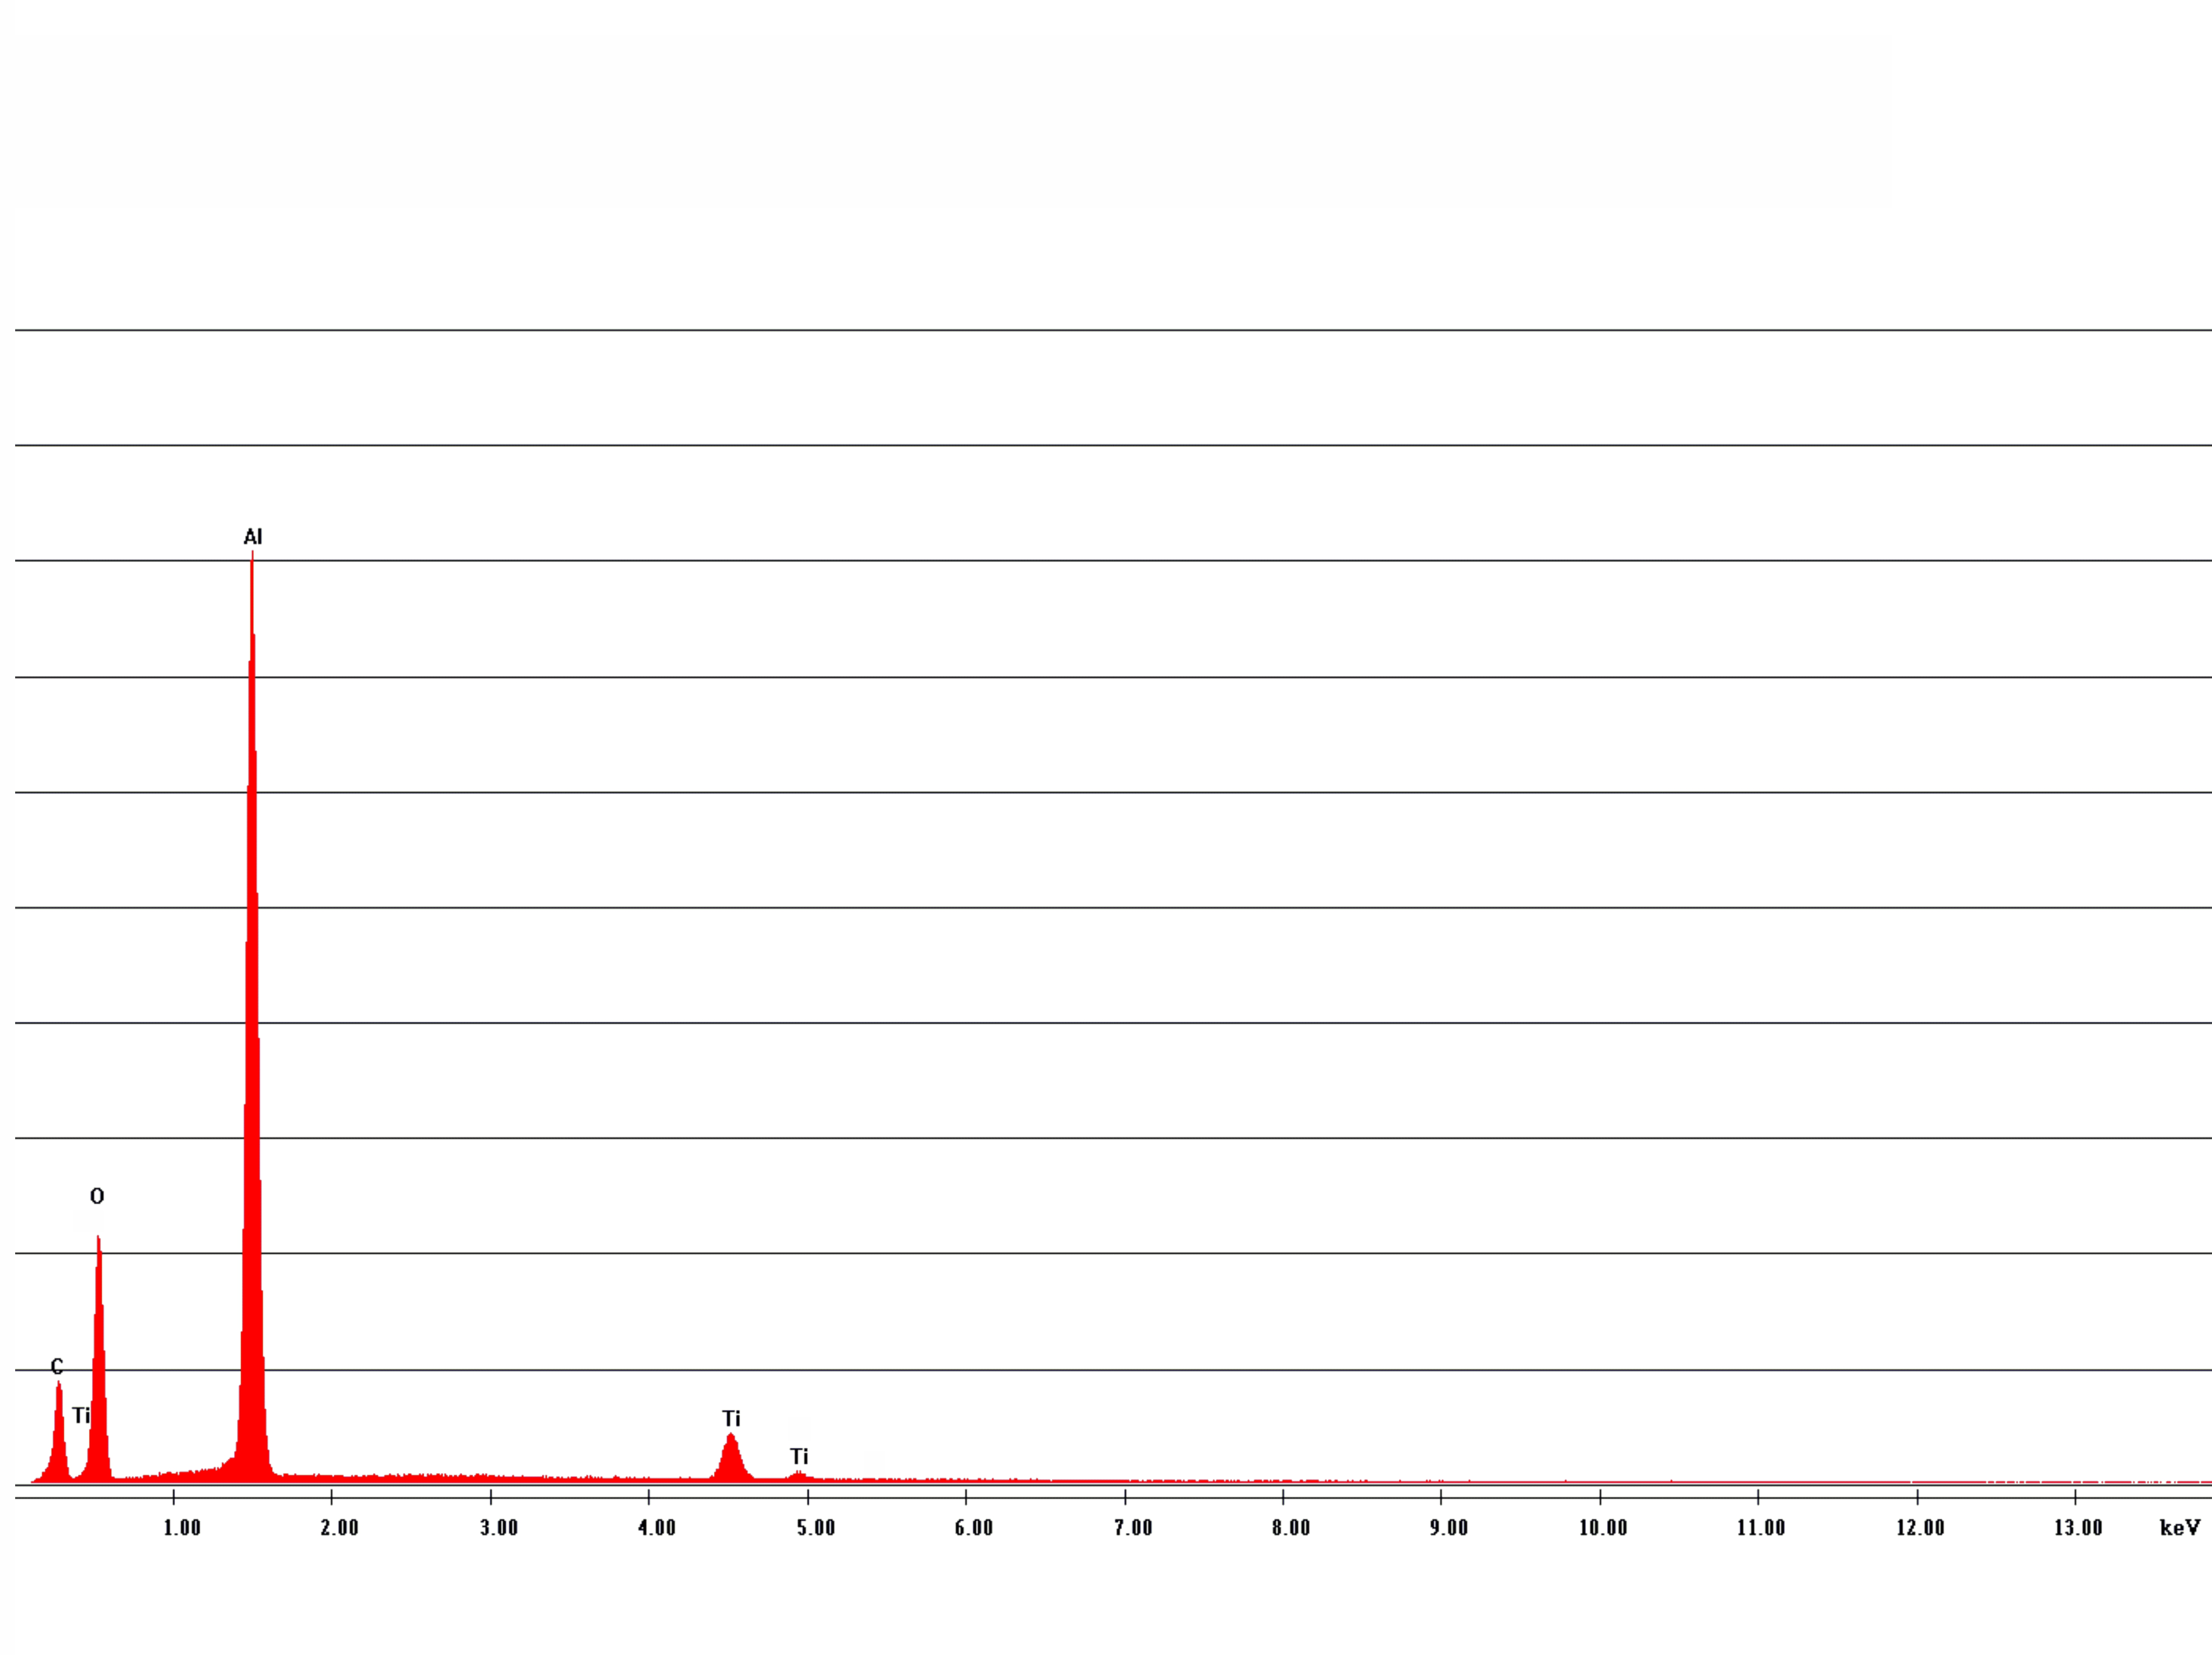
\includegraphics[width =\textwidth,height=5.3cm]{./figures/edx2.png}
	\end{center}
	\caption{EDX-Analyse der Keramikprobe an Position 2~\cite{zankel_serie_nodate}
	}\label{fig:position2}
\end{figure}
\begin{figure}[H]
	\begin{center}
		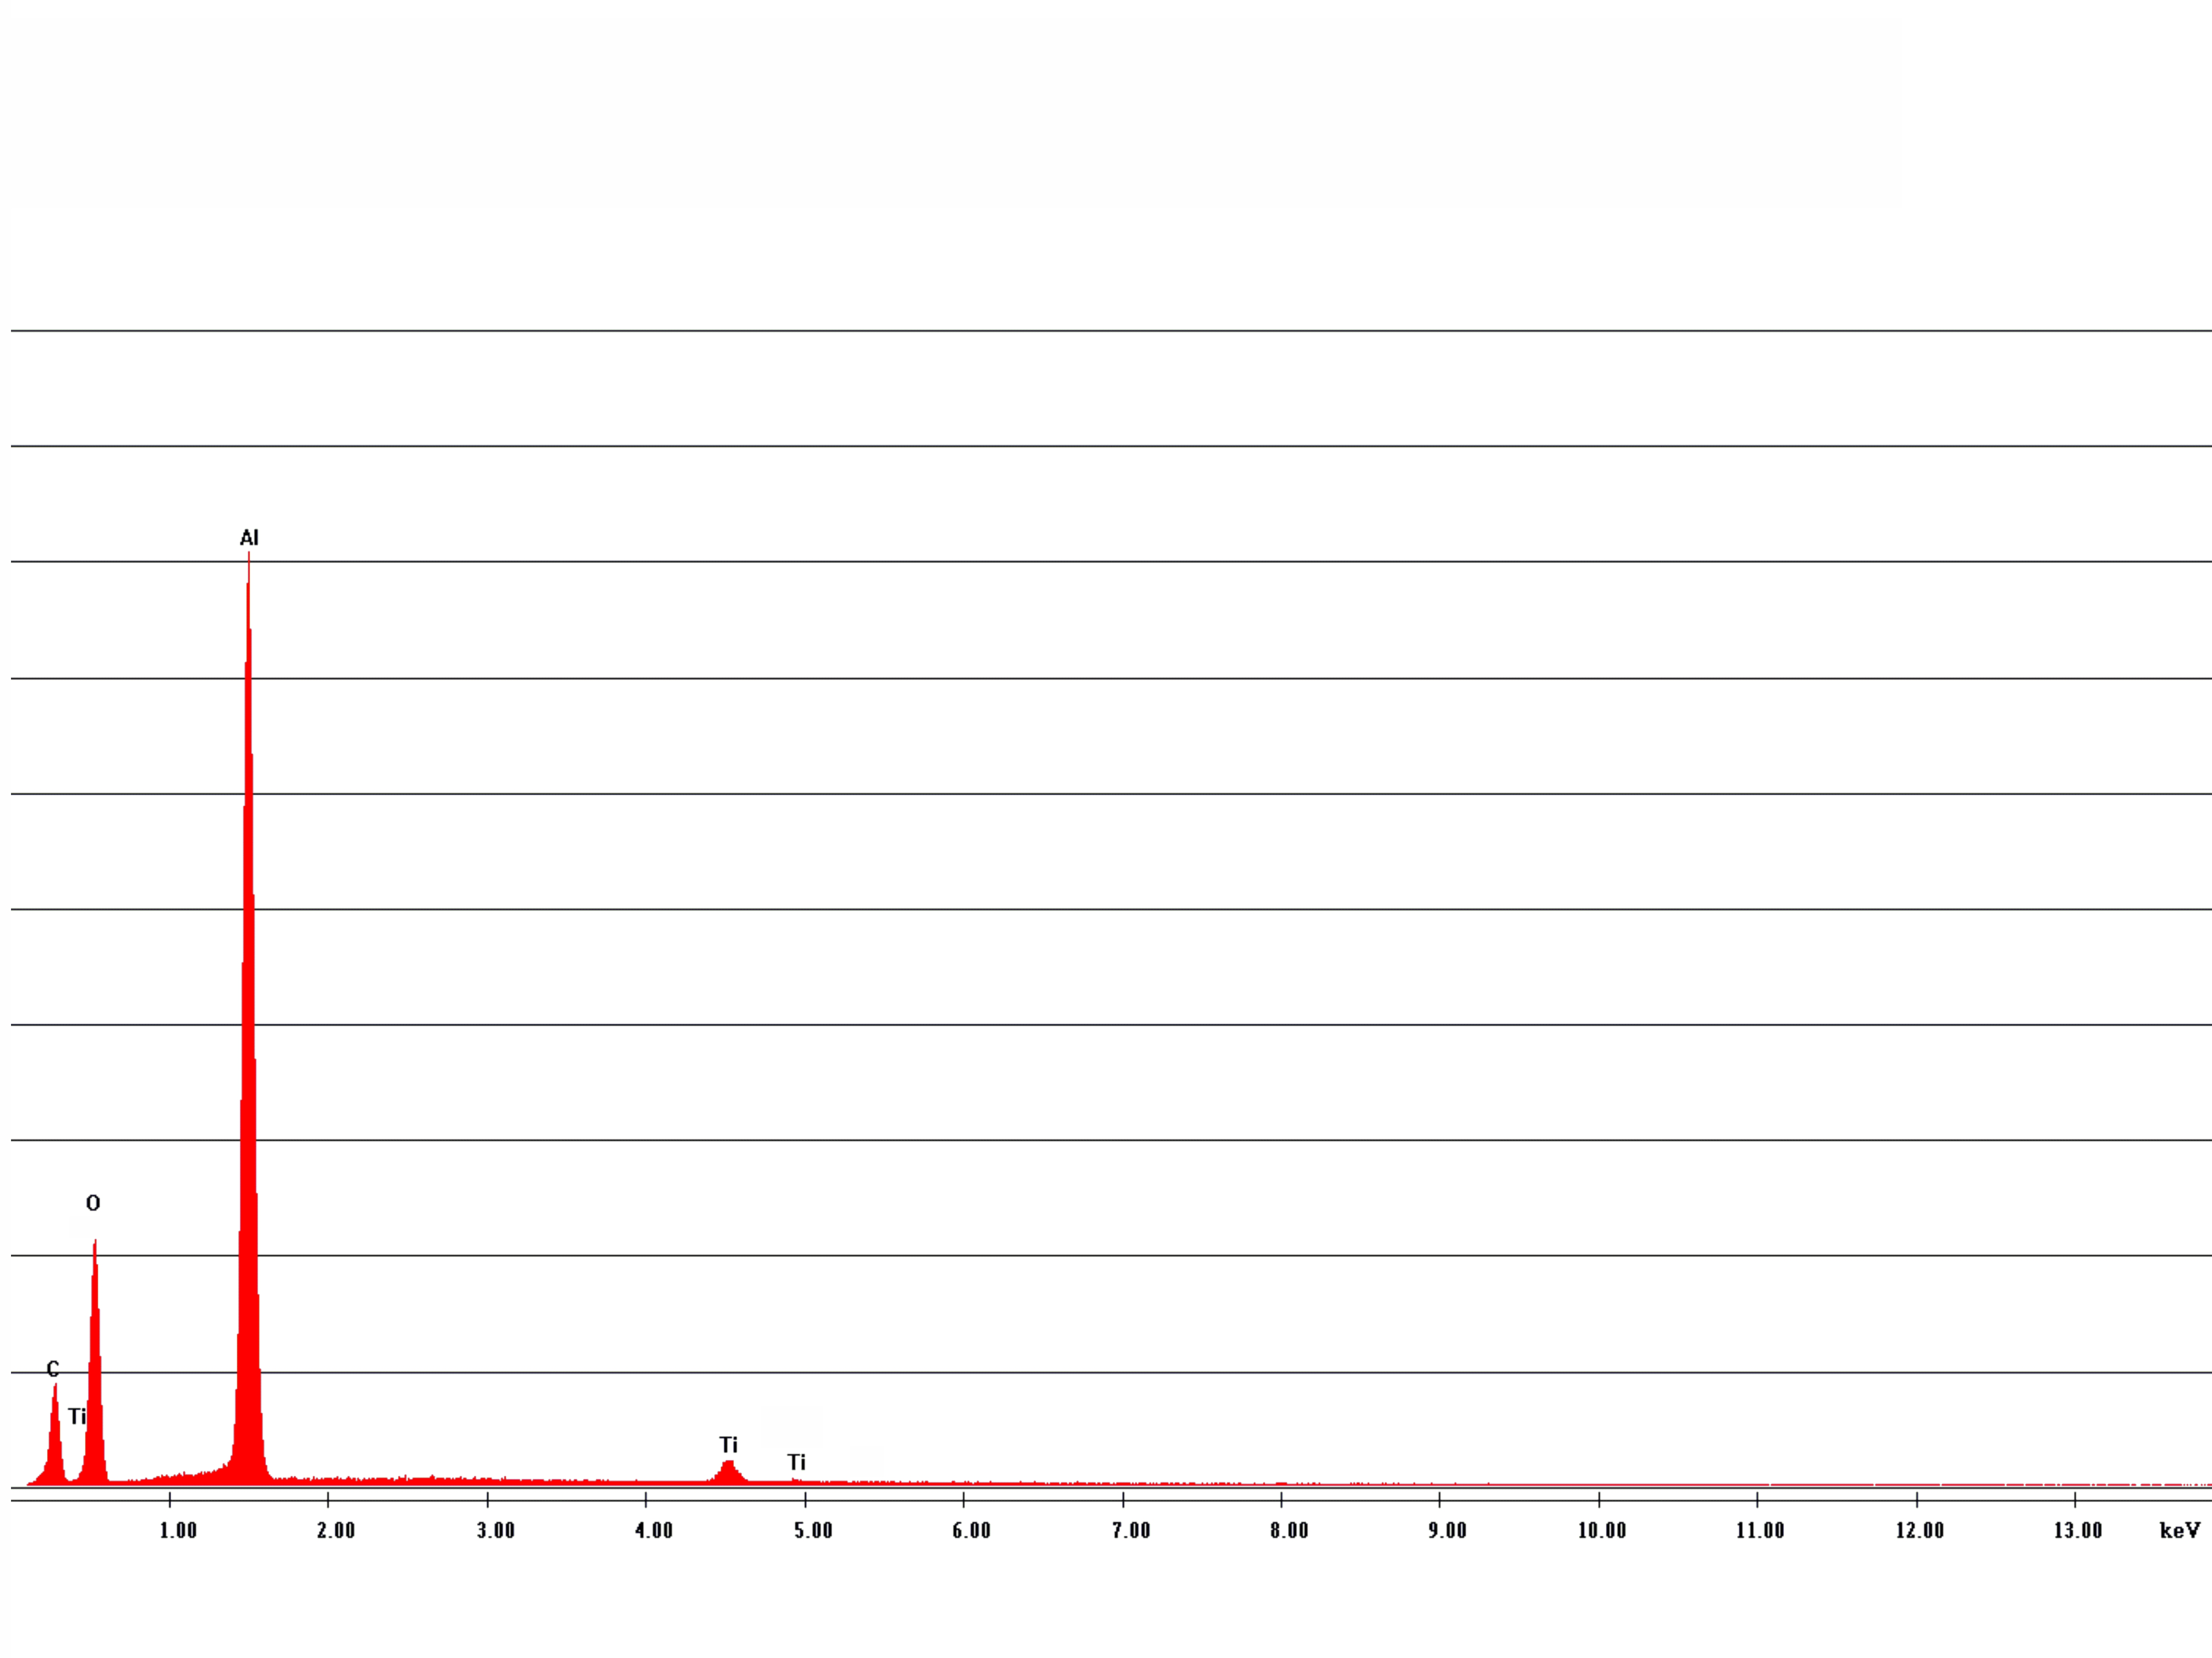
\includegraphics[width =\textwidth,height=5.3cm]{./figures/edx3.png}
	\end{center}
	\caption{EDX-Analyse der Keramikprobe an Position 3~\cite{zankel_serie_nodate}
	}\label{fig:position3}
\end{figure}
\begin{figure}[H]
	\begin{center}
		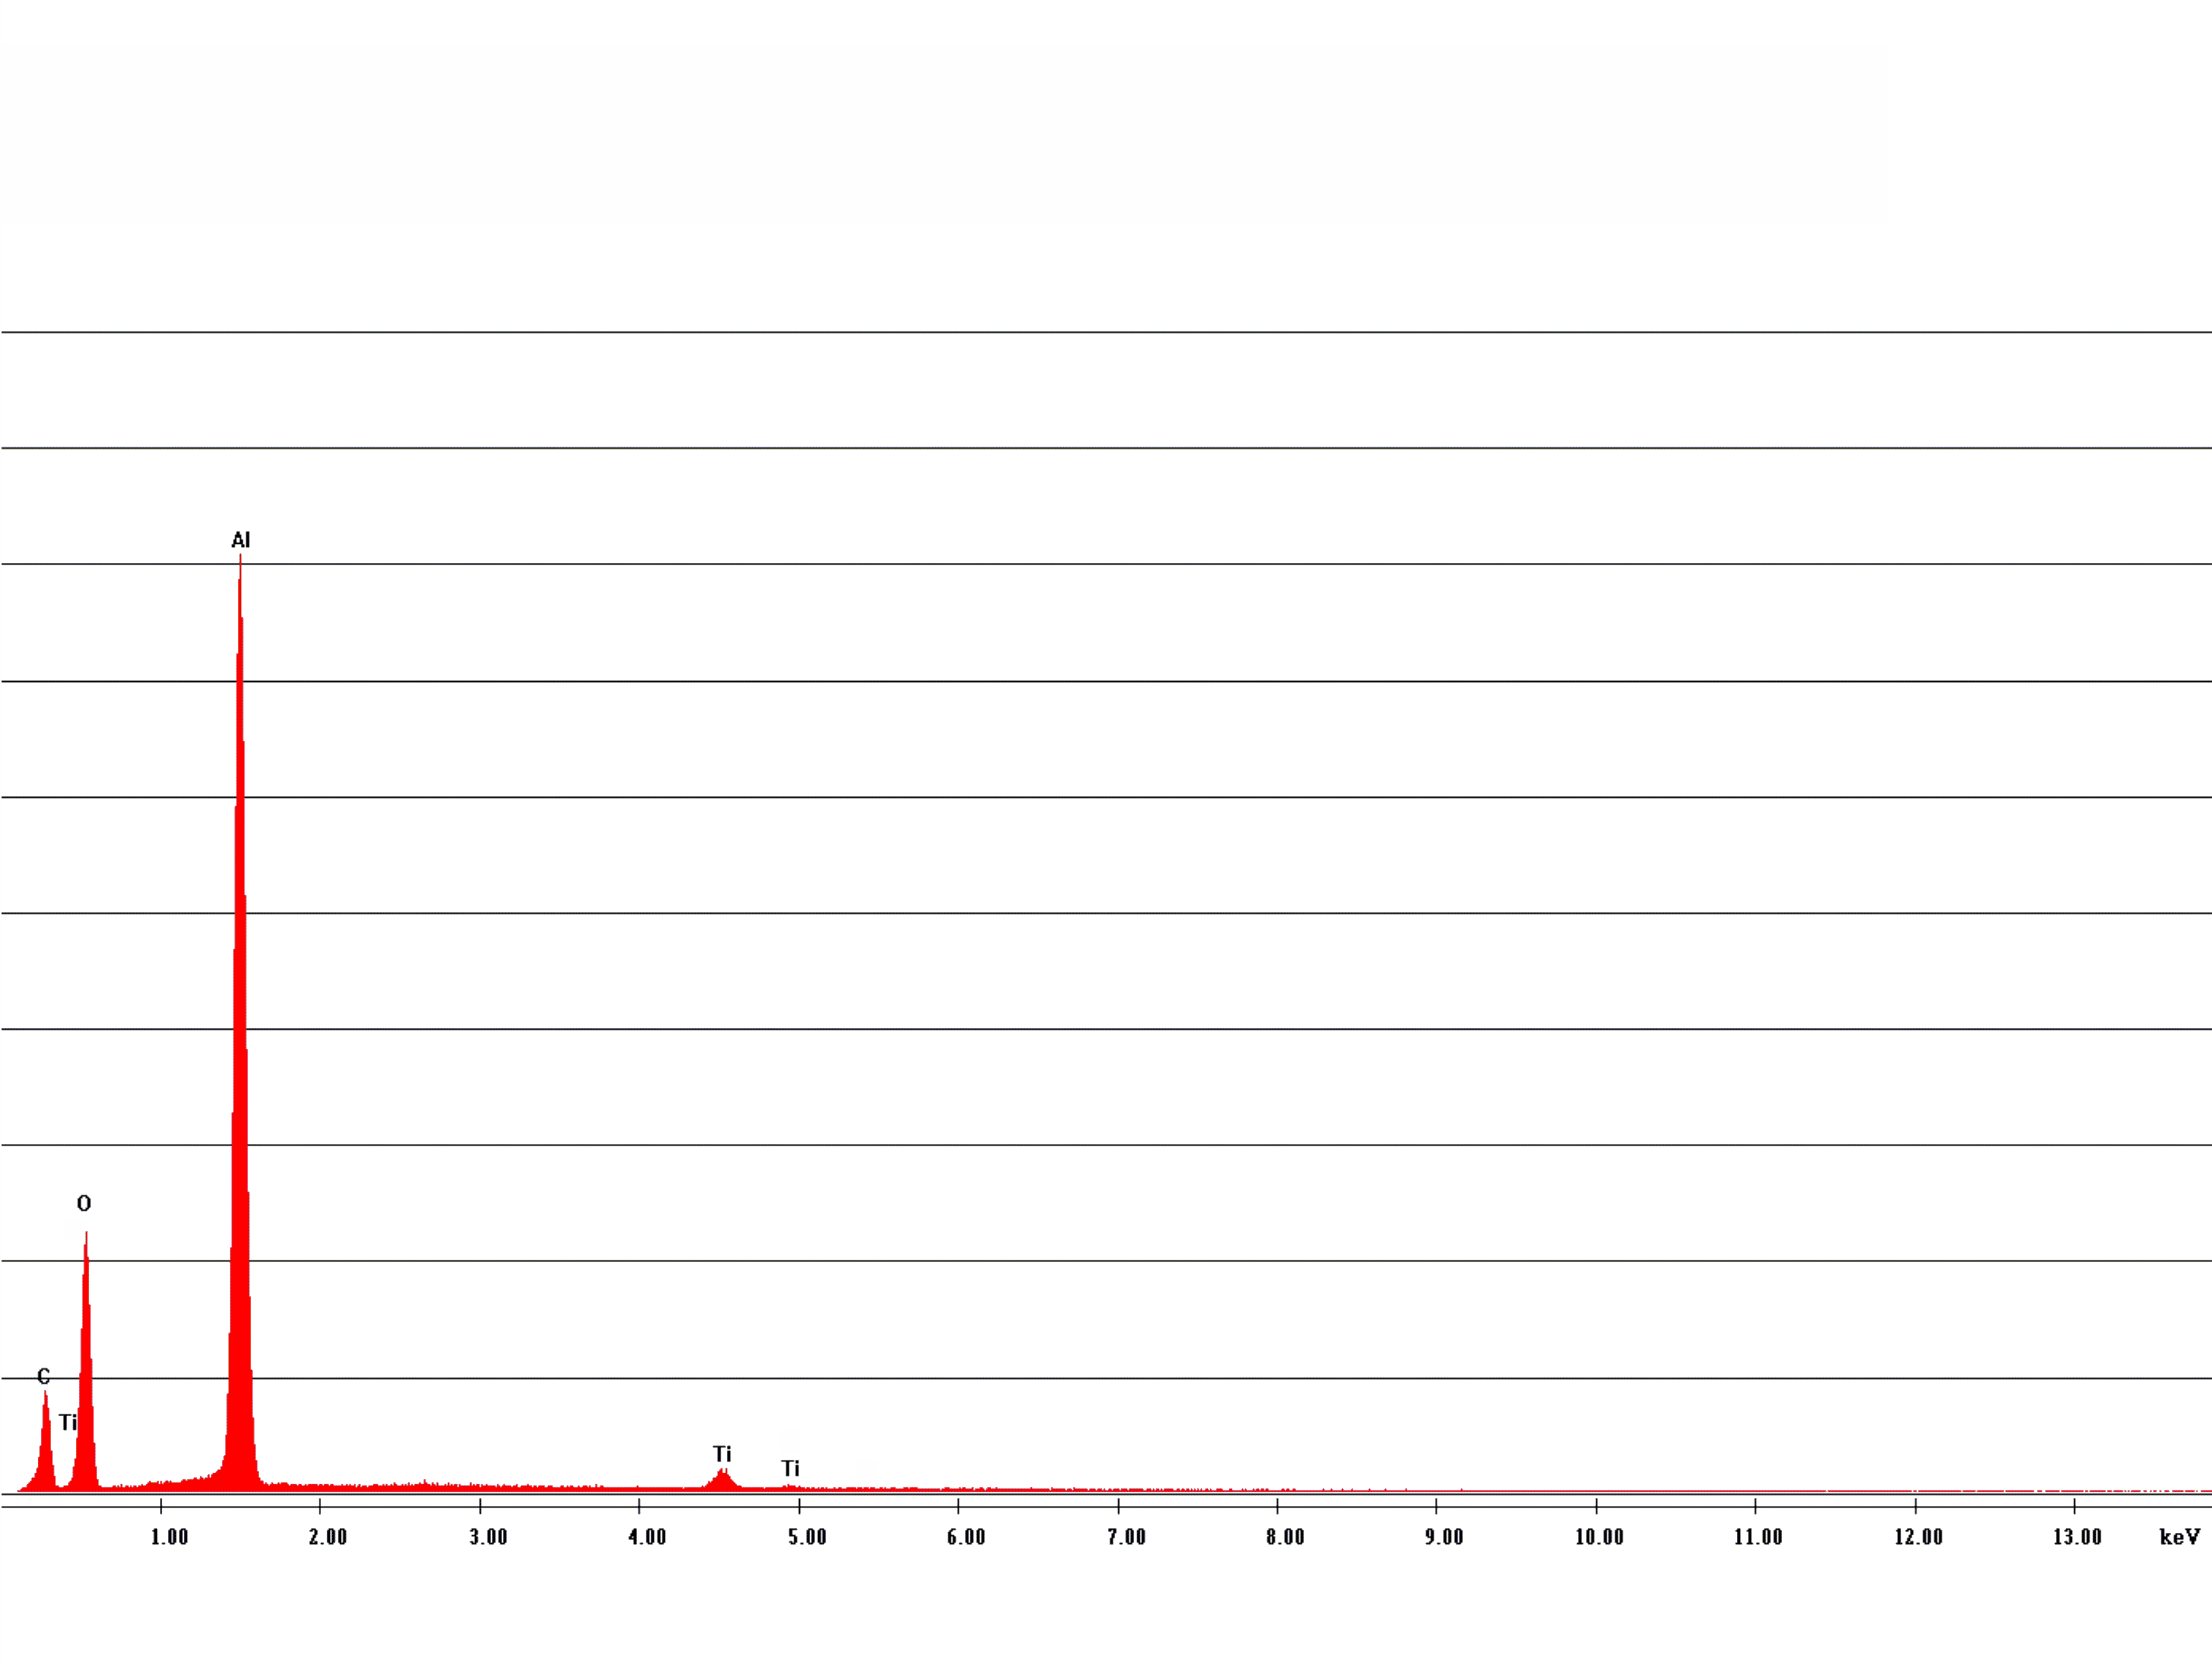
\includegraphics[width =\textwidth,height=5.3cm]{./figures/edx4.png}
	\end{center}
	\caption{EDX-Analyse der Keramikprobe an Position 4~\cite{zankel_serie_nodate}
	}\label{fig:position4}
\end{figure}
\begin{figure}[H]
	\begin{center}
		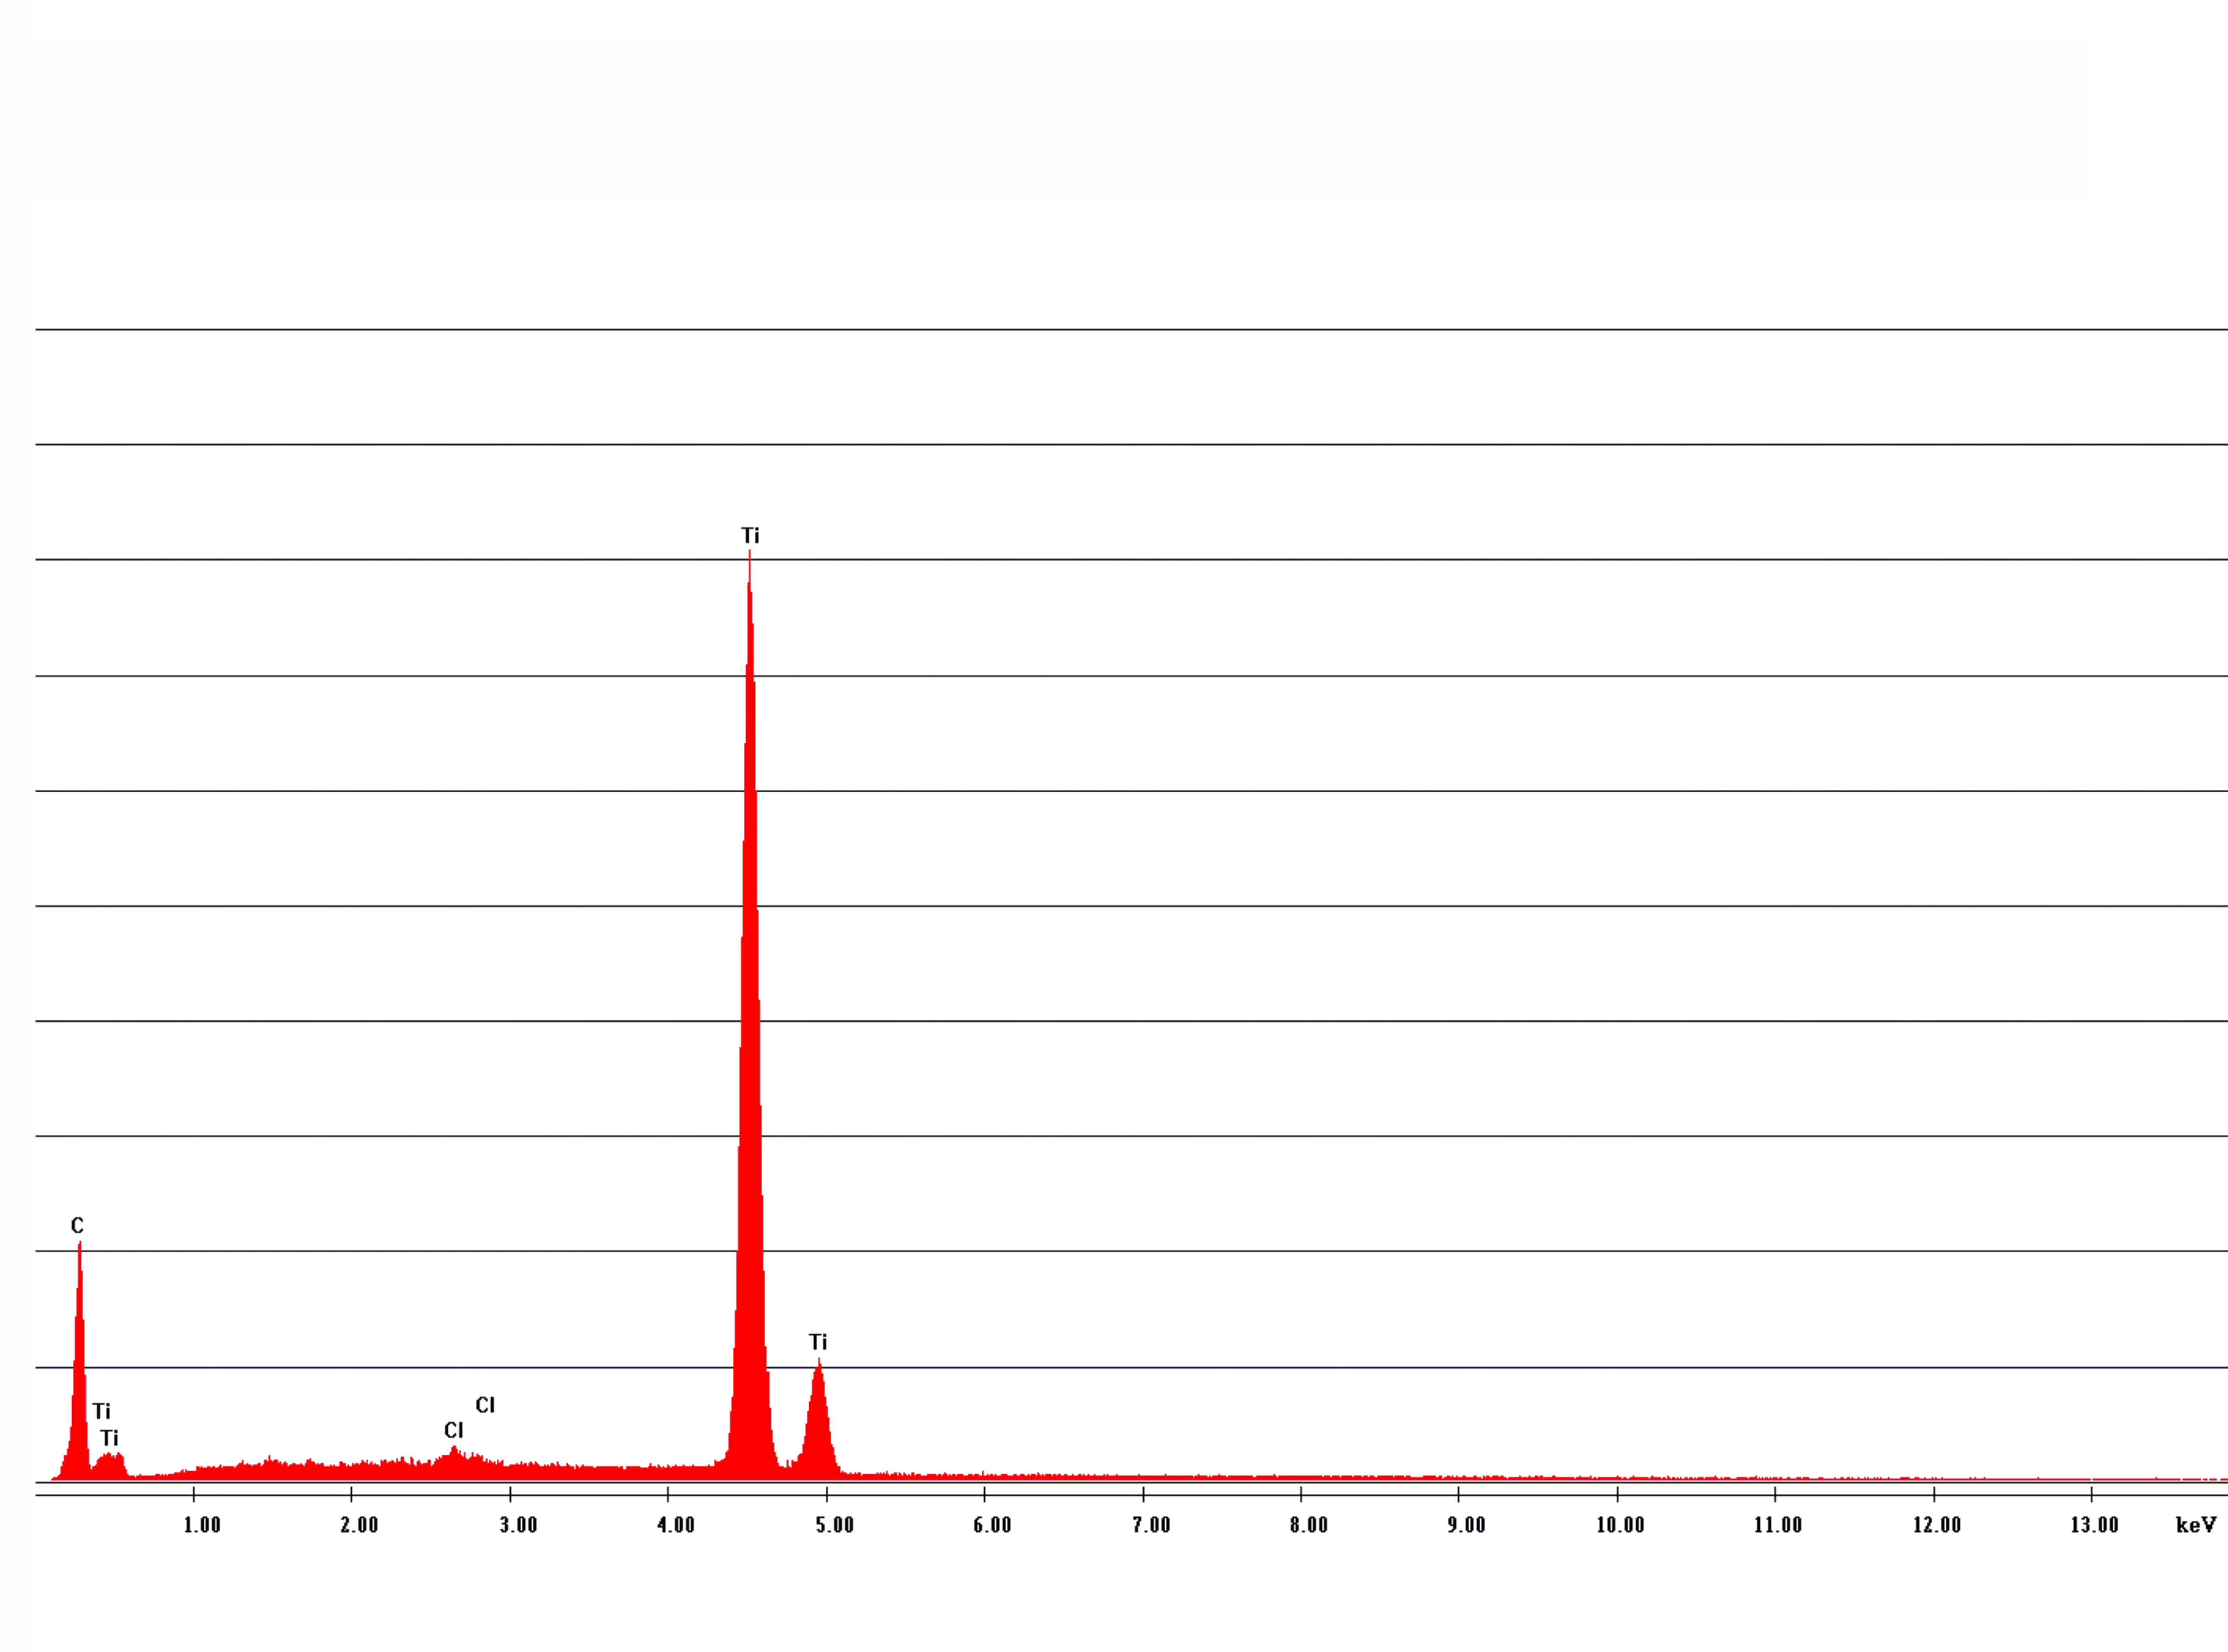
\includegraphics[width =\textwidth,height=5.3cm]{./figures/beschichtung.png}
	\end{center}
	\caption{EDX-Analyse der Beschichtung~\cite{zankel_serie_nodate}
	}\label{fig:beschichtung}
\end{figure}
\begin{figure}[H]
	\begin{center}
		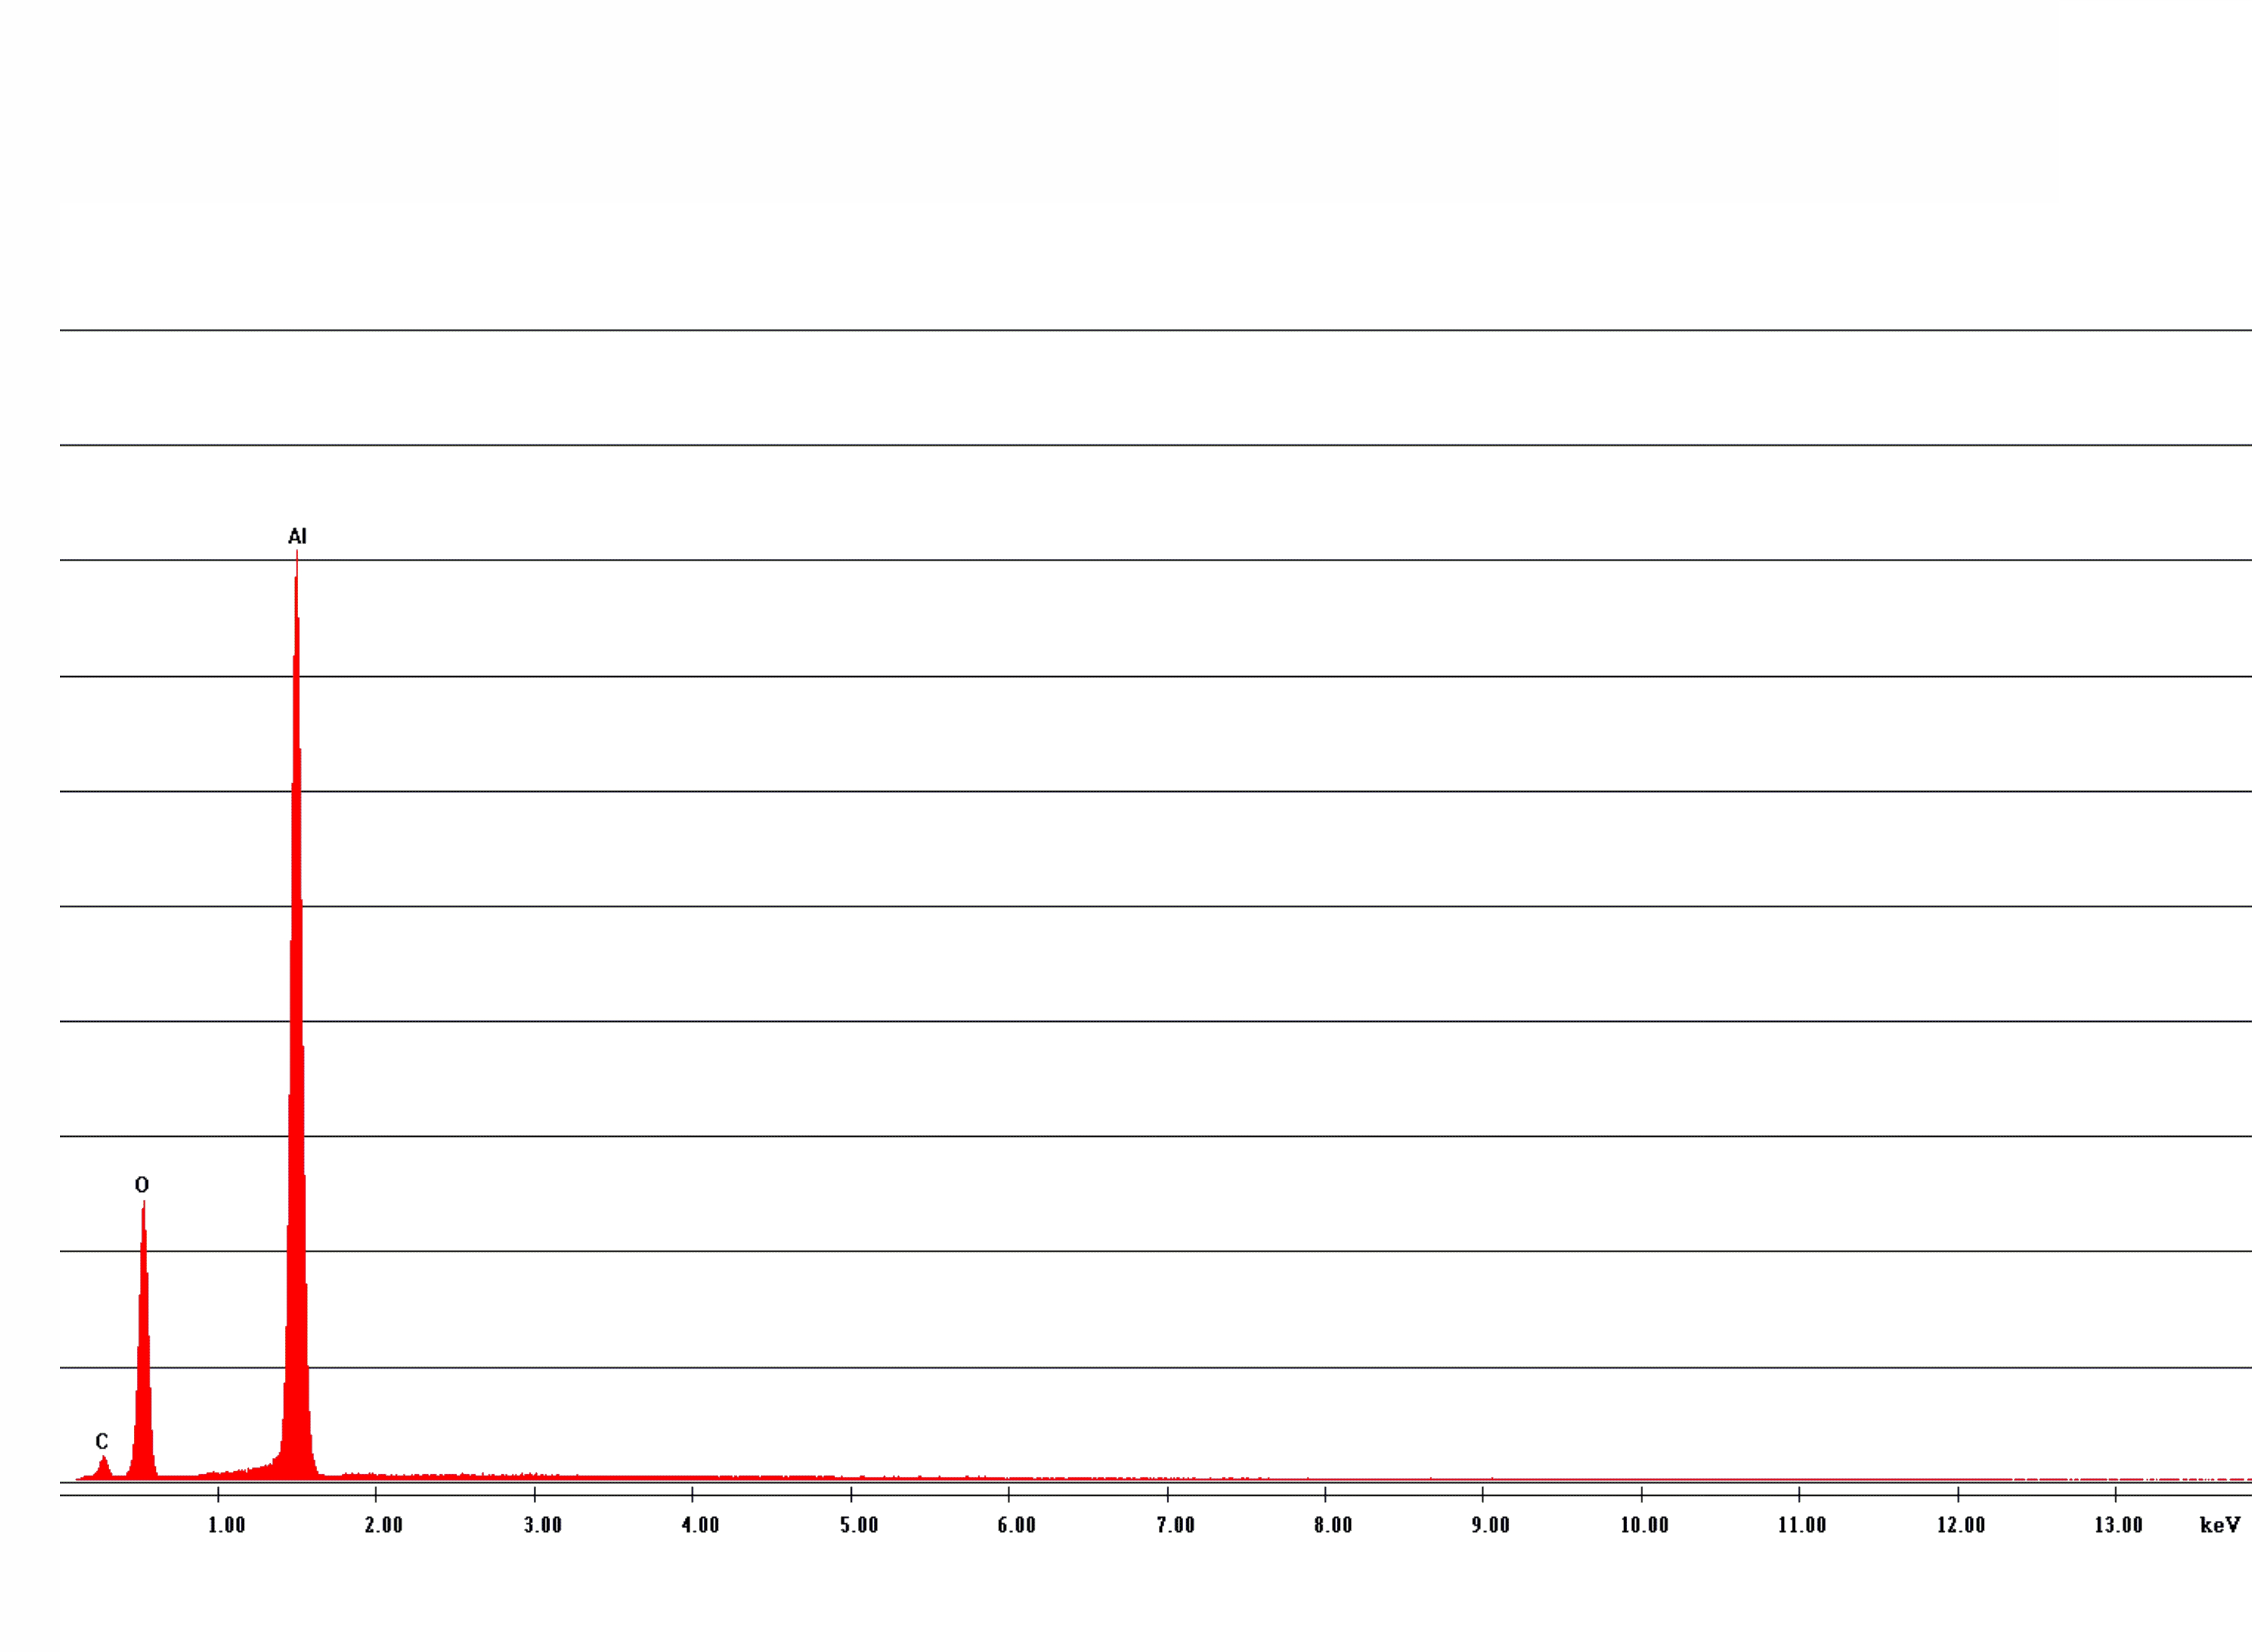
\includegraphics[width =\textwidth,height=5.5cm]{./figures/keramik.png}
	\end{center}
	\caption{EDX-Analyse der Keramikprobe ohne Beschichtung~\cite{zankel_serie_nodate}
	}\label{fig:keramik}
\end{figure}

Beim Vergleich der einzelnen Positionen wird klar ersichtlich, dass der
Ti-Anteil, welcher nach Vergleich mit \autoref{fig:beschichtung} klar der
Beschichtung geschuldet ist, abnimmt, je weiter man sich in das Innere der
Probe bewegt. Dies deckt sich auch mit der Erwartung, da es logisch ist, dass
die Beschichtung etwas in die Probe eindringt, der Anteil aber geringer wird,
je weiter man sich vom Rand wegbewegt, jedoch nie ganz verschwindet.

\section{Quantitative EDX-Analyse}

Mithilfe der EDX-Analyse kann auch eine quantitative Aussage über eine Probe
getroffen werden. Dazu wird eine 10 c-Münze als Probe in den Aufbau gegeben und
die EDX-Analyse durchgeführt. Bei der Wahl der Position ist darauf zu achten,
eine Stelle auszuwählen, an der möglichst keine Verunreinigungen und eine
glatte Oberfläche vorliegen, wie in \autoref{fig:munze} sichtbar. Die Analyse
wurde mithilfe von 2 verschiedenen Detektoren und Programmen durchgeführt. Das entsprechende
Ergebnis ist auch in \autoref{fig:qualitativ1} und~\ref{fig:qualitativ2} ersichtlich.

\begin{figure}[H]
	\begin{center}
		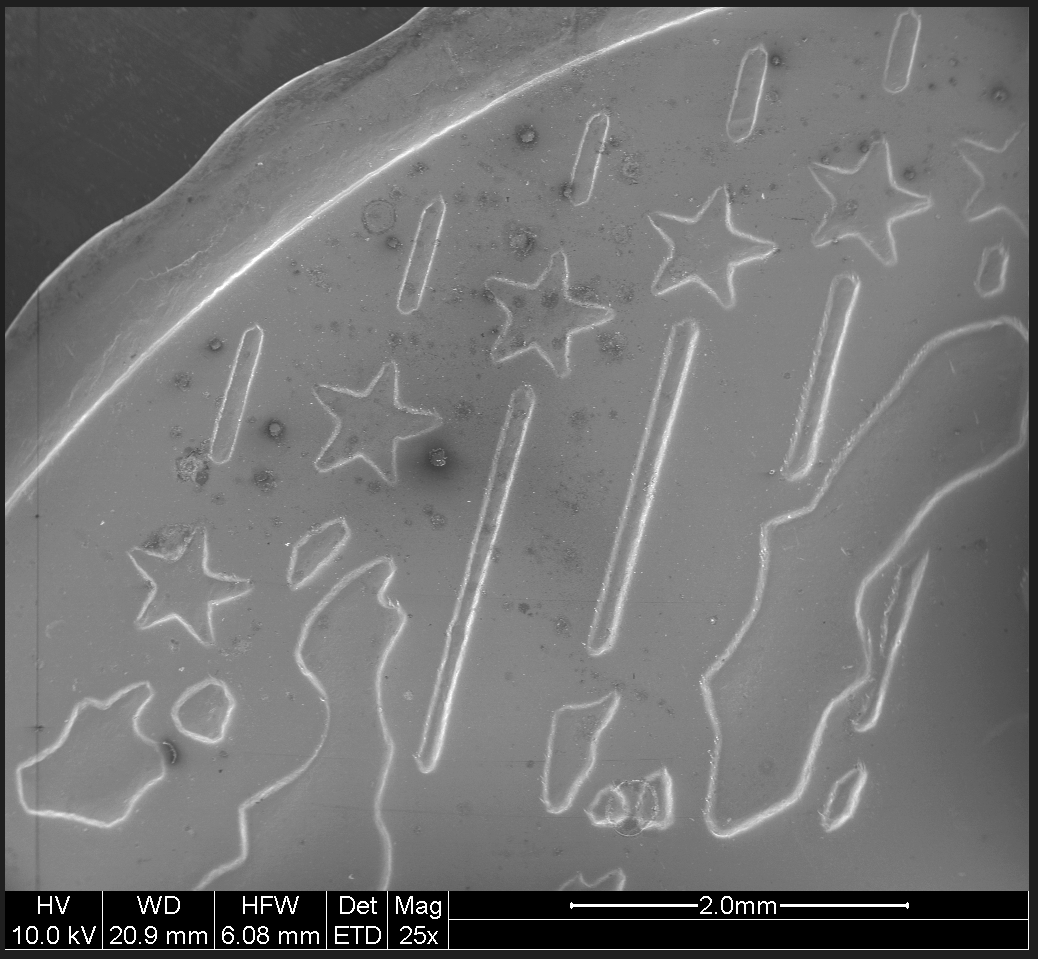
\includegraphics[width =0.5\textwidth]{./figures/munze.png}
	\end{center}
	\caption{SE-Bild der Münzoberfläche~\cite{zankel_rasterelektronenbild_nodate}
	}\label{fig:munze}
\end{figure}

\begin{figure}[H]
	\begin{center}
		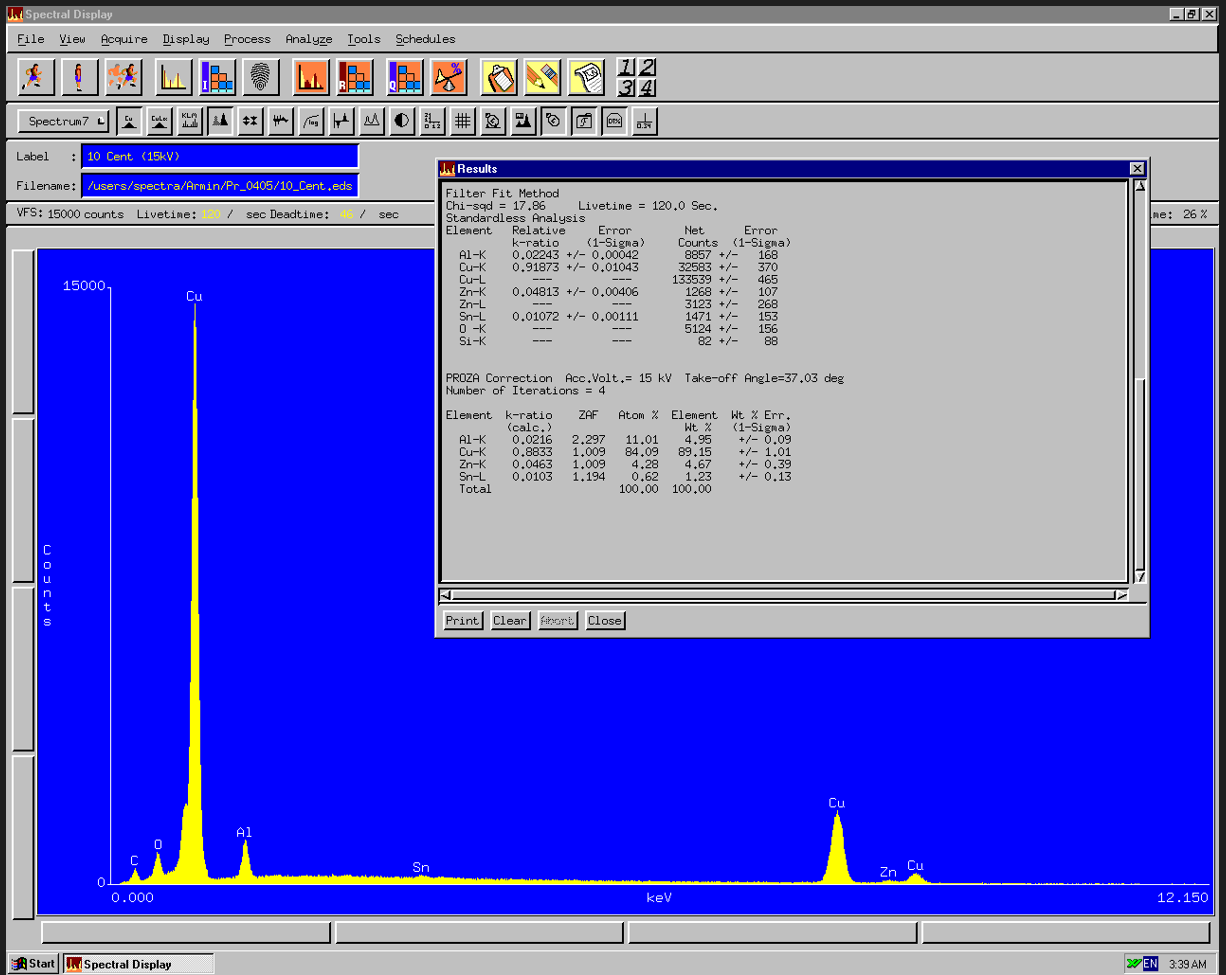
\includegraphics[width=\textwidth]{./figures/qualitativ1.png}
	\end{center}
	\caption{Erzeugtes Spektrum der Münzzusammensetzung~\cite{zankel_quantitative_nodate}
	}\label{fig:qualitativ1}
\end{figure}

\begin{figure}[H]
	\begin{center}
		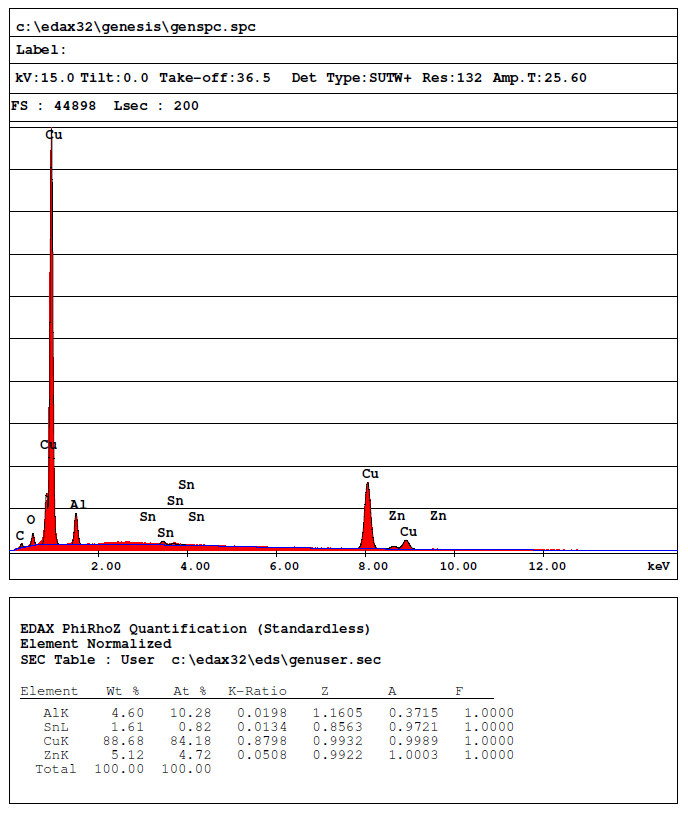
\includegraphics[width=\textwidth]{./figures/qualitativ2.png}
	\end{center}
	\caption{Anderes erzeugtes Spektrum der Münzzusammensetzung~\cite{zankel_quantitative_nodate}
	}\label{fig:qualitativ2}
\end{figure}

Die so erhaltenen Zusammensetzungen sind in folgender
\autoref{tab:zusammensetzung} den entsprechenden Literaturwerten
aus~\cite{noauthor_amtsblatt_2001} gegenübergestellt.

\begin{table}[H]
	\caption[Gegenüberstellung der erhaltenen Zusammensetzung aus der EDX-Analyse der 10 c-
		Münze] {Gegenüberstellung der erhaltenen Zusammensetzung aus der EDX-Analyse der
		10 c-Münze                                                   \\
		Al $\dots$ Aluminium                                         \\
		Cu $\dots$ Kupfer                                            \\
		Zn $\dots$ Zink                                              \\
		Sn $\dots$ Zinn                                              \\
		$P_\text{m1} \dots$ erhaltener prozentualer Anteil mit Detektor 1 \\
		$P_\text{m2} \dots$ erhaltener prozentualer Anteil mit Detektor 2 \\
		$P_\text{lit} \dots$ erhaltener prozentualer Anteil laut Literatur~\cite{noauthor_amtsblatt_2001}
	}
	\begin{center}
		\begin{tabular}{|l|l|l|l|}
			\hline
			\textbf{Element} & $P_\text{m1}$ / \%   & $P_\text{m2}$ / \%   & $P_\text{lit}$ / \% \\ \hline
			Al               & \SI{4.95(9)}{}  & \SI{4.60(5)}{}  & \SI{5}{}       \\ \hline
			Cu               & \SI{89.2(11)}{} & \SI{88.68(5)}{} & \SI{89}{}      \\ \hline
			Zn               & \SI{4.6(4)}{}   & \SI{5.12(5)}{}  & \SI{5}{}       \\ \hline
			Sn               & \SI{1.23(13)}{} & \SI{1.61(5)}{}  & \SI{1}{}       \\ \hline
		\end{tabular}
	\end{center}\label{tab:zusammensetzung}
\end{table}

Ein Vergleich der erhaltenen Ergebnisse mit den entsprechenden Literaturwerten
zeigt, dass die Literaturwerte nicht im Fehlerintervall der durch die Analyse
erhaltenen Werte enthalten sind, jedoch in der gleichen Größenordnung liegen.
Es kann auch festgestellt werden, dass die mit Detektor 1 erhaltenen Werte
meist näher an den entsprechenden Literaturwerten liegen. Eine allgemeine
Aussage kann hier jedoch nicht getroffen werden, da jeweils nur eine einzige
Position betrachtet wurde und die Literaturwerte sich auf die gesamte Münze
beziehen.

Allgemein kann festgehalten werden, dass die EDX-Analyse sehr gut geeignet ist,
um einen groben Überblick über das Vorkommen und die Häufigkeiten von
gewissen Elementen in einer Probe zu bekommen.

\newpage
\section{Zusammenfassung}

Rasterelektronenmikroskopie ist ein sehr bedeutendes Themengebiet, welches ein
breites Anwendungsspektrum besitzt. Im Rahmen des Praktikums durften wir uns
zunächst mit dem Rasterelektronenmikroskop vertraut machen. Dann wurde eine
Polypropylen-Probe in Hinblick auf beschichtete und unbeschichtete Stellen
betrachtet und festgestellt, wie sich die Variation der Beschleunigungsspannung
auf das entstehende Bild auswirkt. Mithilfe einer Keramikprobe wurde der
Unterschied und die Anwendung zwischen SE- und BSE-Abbildungen in Erfahrung
gebracht und die Schichtdicke einer Schicht auf der Keramikprobe vermessen. Zum Abschluss wurde
noch eine qualitative sowie eine quantitative EDX-Analyse durchgeführt, um die
Elemente sowie die prozentuale Zusammensetzung einer Probe zu untersuchen.

\printbibliography{}

%todo bei zitationen statt herbert -> reingruber

%\appendix
%\renewcommand{\thesection}{\Roman{section}}
%\section{Anhang}

%Hier werden, wie von der Aufgabenstellung verlangt, nochmals alle
%Vorbereitungsunterlagen und die Daten zu den Münzen angeführt.

%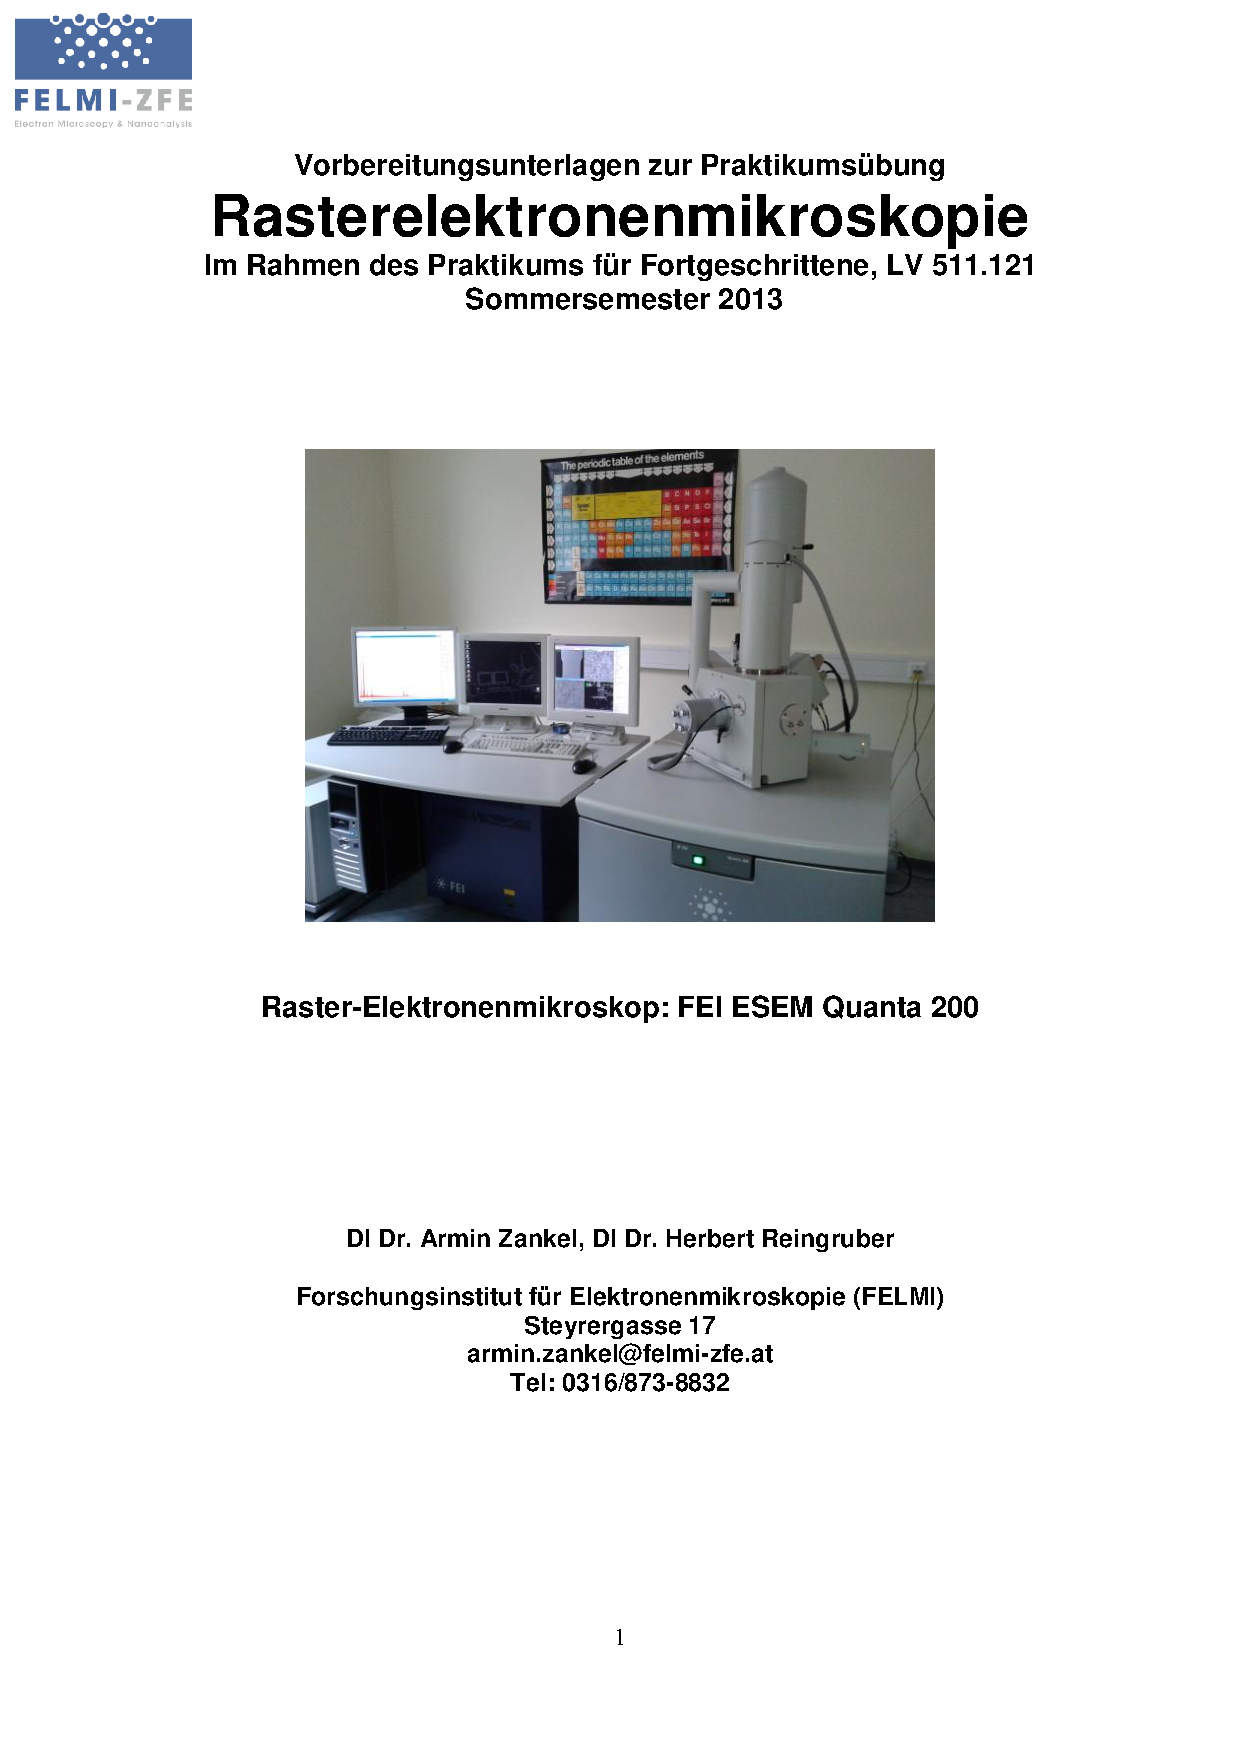
\includepdf[pages=-]{./pdfs/Praktikumsunterlagen_REM_LV_511.121_2013.pdf}
%\includepdf[pages=-]{./pdfs/Amtsblatt_Euromünzen.pdf}

\end{document}
